%Sample of text file to include all the documents
\documentclass[12pt,LUDisStyle,twosided]{book}
\usepackage[hang,small,bf]{caption}
\usepackage{LUDisStyle}
\usepackage{graphicx}
\usepackage{subfigure}
\usepackage{amsmath}
\usepackage{amssymb}
\usepackage{amsthm}
\usepackage{verbatim}
\usepackage{multirow}
\usepackage{float}
\usepackage[square,numbers]{natbib}
\renewcommand{\topfraction}{0.95}
\renewcommand{\textfraction}{0.05}
\renewcommand{\floatpagefraction}{0.85}
\addtolength{\belowcaptionskip}{10pt}
\newcommand{\mc}{\mathcal}

\begin{document}
\pagestyle{plain}
\pagenumbering{roman}
\dissertationtrue
\thispagestyle{empty}%

	\vskip0.5in%

	\begin{center}

		\LARGE Model fidelity and its impact on power grid resource planning under high renewable penetration

	\end{center}

	\vfill

	\begin{center}

		\rm by \\
		
                         \vfill
                 
		Daniel Xavier Wolbert \\

	\end{center}

	\vfill

	\begin{center}

		\rm A Thesis \\

		Presented to the Graduate Committee \\

		of Lehigh University \\

		in Candidacy for the Degree of \\

		Master of Science \\

		in \\

		Industrial and Systems Engineering

	\end{center}

	\vfill

	\begin{center}

		Lehigh University \\

		05/2106 \\

	\end{center}\vskip.5in
	
	\newpage

%put copyright info on second page
\vspace*{\fill}
\begin{center}
Copyright\\
Daniel Xavier Wolbert
\end{center}
\newpage
%Sample signature page

\thispagestyle{plain}

Approved and recommended for acceptance as a thesis in partial fulfilment of the requirements for the degree of Master of Science.
\\
\\
Daniel Xavier Wolbert \\
Model fidelity and its impact on power grid resource planning under high renewable penetration

\vspace{.1in}

\begin{tabular}{l}
\\
\hline
\textbf{05/06/2016 \ \ \ \ \ \ \ \ \ \ \ \ \ \ \ \ \ \ \ }
\end{tabular}

\begin{flushright}
\begin{tabular}{l}
\\
\hline
\textbf{Robert H. Storer}, Thesis Director, Chair \\ 
\textbf{(Must Sign with Blue Ink)}
\end{tabular}

\vspace{.05in}

\end{flushright}

\begin{tabular}{l}
\\
\hline
\textbf{Accepted Date \ \ \ \ \ \ \ }
\end{tabular}


\begin{flushright}
\begin{tabular}{l}
Committee Members \ \ \ \ \ \ \ \ \ \ \ \ \ \ \ \ \ \ \ \ \ \ \ \ \ \
\\ 
\\
\\
\hline
\textbf{Tamas Terlaky}, Chairperson of Department\\
\\ 
\\
\\

\end{tabular}
\end{flushright}
\newpage
\chapter*{Acknowledgements}

I would like to thank the Industrial and Systems Engineering department at Lehigh University to provide me help and guidance. A special thanks to Prof. Robert H. Storer to be my supervisor and give me the necessary support to achieve my objectives.

Also, I would like to thank Dr. Dimitri Papageorgiou and his team to help me with all the data and necessary technical support, as well as professional advices.

I would like to thank the CAPES on behalf of the brazilian government to sponsor me and provide me everything necessary to achieve my goals. Finally, I would like to thank my family, my future wife and my friends in US and Brazil for their continuous moral support and positive energies. I could not express in words how grateful I am.
\tableofcontents
\nopagebreak
\addcontentsline{toc}{chapter}{List of Tables}
\listoftables
\addcontentsline{toc}{chapter}{List of Figures}
\listoffigures
\newpage
\pagestyle{plain}
\pagenumbering{arabic}
\addcontentsline{toc}{chapter}{Abstract}
Renewable generation resources are one of the biggest trends emerging into the power systems world. The variability of these power sources brings challenges in terms of planning, reliability and feasibility factors. Classical formulations of Optimal Power Flow systems tries to generate power system at minimal costs, considering devices and transmission constraints.

This work evaluates the impact of different levels of green energy in terms of the two most common optimization models in power systems planning: the Unit Commitment and Economic Dispatch, under different time modelling and transmission assumptions. This thesis built a full user-friendly tool in AIMMS with 4 datasets based on the IEEE RTS-96 Test Cases with Wind and Solar profiles incorporated from the state of Texas, and it is going to be available to the academic community for power systems planning research purposes, with capacity to expand.

The analysis discusses that there, under high renewable resource penetration levels more factors has to be considered in the planning, such as ramping, under and over generation, storage behaviour, transmission line limits and start-up, shut-down profiles. It is also suggested that, under deep sub-hourly levels, the classic formulation of unit commitment is not efficient and, therefore is necessary to incorporate new optimization techniques.
\pagestyle{plain}

\chapter{Introduction}

By many accounts, renewables resources will likely play a key role in the electric grid system for many countries in the next decades \cite{rahmangreen}.  Variable renewable energy (VRE) (e.g., wind and solar) have random intermittent output, and thus do not behave like the dispatchable resources used for the vast majority of today's electricity generation. The variability of these sources has led to concerns regarding the reliability of an electric grid that derives a large fraction of its energy from these sources as well as the cost of reliably integrating large amounts of variable generation into the electric grid. To address these concerns, the electricity grid may incorporate additional technologies that provide one or more of the following attributes: fast ramping capabilities, load shifting, demand response, energy storage, and more.   Which technologies and grid configurations prevail are likely to be impacted by several factors including economics (i.e. the costs and benefits of each technology are weighed relative to the other available options), reliability, local and regional policies and other region-specific resource constraints.

Underpinning many of the economic and reliability studies used to assess various technologies are optimization and simulation models.  These models make numerous approximations when determining optimal Economic Dispatch and power flow, the consequences of which are not fully understood, especially with substantially more variable renewable resources and different grid configurations. 

The first goal of this thesis is to investigate and attempt to characterize the subtleties that arise when making certain approximations to model day-ahead and real-time dispatch decisions. The investigated scenarios represent instances of real-world grid configurations on a shorter scale with different levels of renewable resource penetration.

In general, power system models can be classified according to different features, that include:

\begin{enumerate}
\item Time frame: decade, year, hour, sub hour 
\item Scale: global, national, regional, local
\item Deterministic vs stochastic
\item Optimization vs Simulation
\item Algorithmic vs Heuristic
\end{enumerate}

In its current form, the software developed in this thesis considers two of the most prominent optimization models: Economic Dispatch (ED) and Unit Commitment (UC). 

Economic Dispatch (ED) models are often deterministic linear optimization models that attempt to determine the minimum cost output of available generators to meet system load (demand), subject to transmission and operational constraints, in every time period over a fixed time horizon.  These models are typically formulated with a resolution of one hour or less with a short time horizon. Without transmission or operational constraints, ED models are simple to solve. Generators are first sorted in ascending order according to their marginal costs (forming a so-called ``merit-order curve'') and then dispatched in that same order until system load is met. The marginal cost of the final generator needed to meet load determines the system marginal cost, the cost of delivering one additional MWh of energy onto the system.  With transmission, operational, and/or environmental constraints, however, these models require more sophisticated optimization algorithms to determine the optimal generation allocation.  For most representations of transmission constraints, linear optimization models suffice.  For detailed AC transmission formulations, non-convex nonlinear NP-hard models arise. Historically, these models are hard to solve in a practical amount of time, which is one of the reasons Economic Dispatch is so popular with grid planners nowadays.

Unit Commitment (UC) models most often refer to mathematical programs that attempt to schedule generators to meet system load in the future based on some forecast of net load (load minus generation from renewable sources).  Whereas ED models typically assume generator availability has already been determined (and, thus, is an input to an ED model), a UC model must determine on/off decisions for each generator in the fleet in each future time period.  Consequently, UC models are often formulated as mixed-integer linear programs and are more difficult to solve than ED models. Stochastic and robust UC models include an additional layer of complexity by assuming that forecasted parameters are uncertain. The presence of additional binary variables in the model considerably increases the solution time. So, usually UC models are solved for less than a 24 hour horizon, on an hourly level. However, one of the goals for this project is evaluate what happens in terms of solution quality and time when the horizon is bigger and the time granularity is shorter.

A secondary goal of this thesis is the development of an open-source software tool for power systems optimization. Why develop another power systems software tool? There are a number of existing tools available in the power systems community (see the references given in \cite{greenhall:2012}). For example, one of the most popular open-source tools is MatPower \cite{matpower:2011}, which is advertised as a tool "for solving power flow and optimal power flow problems" and thus is not ideal for multi period problems. In addition, one of the major drawbacks of Matlab is that it lacks a user-friendly algebraic modelling interface.  Instead, one must enter constraints as vectors or matrices, which is less natural than the algebraic models that students are taught and practitioners use in the optimization community. Especially for starters, having a user-friendly intuitive tool with a simpler method can be much more powerful than a powerful technical one with a hard interface with which to interact.

The tool developed in this project more closely resembles the work done for Minpower \cite{greenhall:2012},
an open-source toolkit coded in Python that relies on Pyomo \cite{pyomo:2012}. AIMMS provides a free academic license and thus can facilitate power systems optimization and analysis.
It has plug-ins to all major optimization solvers and other features, as well as the ability to easily change and expand one's models to study new systems and configurations.

\chapter{Literature Review}

As mentioned previously, power planning is a popular topic in Operations Research, and it is becoming even more challenging with the increase of wind and solar in the grid. \citeauthor{cain} \cite{cain} divides power flow formulations into 3 major categories: Power Flow (PF), Economic Dispatch (ED) and Optimal Power Flow (OPF) and describe them based on the assumptions and operational constraints, as shown in Table \ref{table:PowerSystemsCat} .

% Please add the following required packages to your document preamble:
% \usepackage{multirow}
\begin{table}[h!]
\centering
\caption{Optimal Power Flow Categories.}
\resizebox{\linewidth}{!}{%
\label{table:PowerSystemsCat}
\begin{tabular}{|l|l|l|l|l|l|l|l|}
\hline
\multirow{3}{*}{Category} & \multirow{3}{*}{Name} & \multicolumn{5}{l|}{Constraints} & Costs \\ \cline{3-8} 
 &  & \multicolumn{2}{l|}{Voltage} & \multirow{2}{*}{Transmission} & \multirow{2}{*}{Contingency} & \multirow{2}{*}{Losses} & \multirow{2}{*}{Generator} \\ \cline{3-4}
 &  & Angle & Magnitude &  &  &  &  \\ \hline
OPF & ACOPF & x & x & x &  & x & x \\ \hline
OPF & DCOPF &  &  & x & x & x & x \\ \hline
OPF & DOPF & x & x & x &  & x &  \\ \hline
OPF & SCED & x &  & x & x & x & x \\ \hline
OPF & SCOPF & x & x & x & x & x & x \\ \hline
PF & PF &  & x &  &  & x & x \\ \hline
ED & ED &  &  &  &  & x & x \\ \hline
\end{tabular}
}
\end{table}


\citeauthor{yamin} \cite{yamin} discusses different techniques to solve the Unit Commitment and Economic Dispatch problems, categorizing them in deterministic, heuristic or stochastic, pointing out the computational challenges and the quality of results for each one of them . 

\citeauthor{bertsimas} \cite{bertsimas} proposes a two-stage robust optimization to mitigate demand and variability uncertainties to solve UC when renewable resources are a major element in the field. The authors point out the advantages of the method by comparing to traditional planning methods. 

\citeauthor{padhy} \cite{padhy} formulates the Unit Commitment problem as a general optimization problem and presents a bibliographical survey of the main techniques in the last 30 years, from exhaustive methods such as priority listing, dynamic programming, mixed integer-programming up to complex heuristics like fuzzy programming, genetic algorithms and evolutionary programming. However the authors state that further testing is required for those methods.

\citeauthor{connolly} \cite{connolly} review 68 tools to power grid planning with renewable resources, discussing, at the end, goals, limitations and features of 37 tools. The authors emphasize that, although all the tools are essential to accurate power planning with renewable resources, there is no perfect tool, and it should be chosen accordingly to project goals, data limitations, horizon and other features. 


\citeauthor{kassakian} \cite{kassakian} discuss the main changes and challenges in the power system for future years. One of important changes is the increase of VRE, that might have substantial impacts in operating costs, primarily due to the necessity of more reserve generation with different time responses. To mitigate this increase in the operating costs, 3 suggestions were proposed: improve wind and solar forecasting techniques, expand the cooperation and interconnections among regions and reduce decision horizon and resolution levels, to capture more realistic ramping and reserve effects.

\citeauthor{palmintier} \cite{palmintier} study the impact of UC models with expansion planning, highlighting that ignoring operating constraints on expansion planning with VRE could provide higher operating costs and emissions. \citeauthor{hargreaves}  \cite{hargreaves} propose a method that combines simulation and stochastic UC to capture precisely the challenges of expanding the capacity with VRE.

Under a scenario where VRE have considerable penetration in the power system, it is necessary to study their impact. \citeauthor{deane} \cite{deane} evaluates the UC and ED results at different temporal resolutions under one year. The authors discuss that sub-hourly resolutions can deal more accurately with non-thermal inflexibilities, renewable demand variabilities and ramping behaviours than one-hour resolution. 

One of the alternatives studied in the literature is the use of storage devices to stock energy when the demand is lower than the capacity and use it on an abrupt peak demand, avoiding the use of conventional generators.  \citeauthor{safaei} \cite{safaei} study different storage technologies and their impact on the emission grid at a 15 minute time resolution, without transmission constraints and forecast errors. The main insights are that cheap storage does not have major impact in the cost of reducing the carbonization, and seasonal storage is not economically justifiable. In the other hand, \citeauthor{harris} \cite{harris} study the viability of seasonal storage by analysing UC results of different storage scenarios and technologies on a city level, concluding that seasonal storage can bring operational benefits and reduce operating costs and fuel emissions at peak load. \citeauthor{dwyer} \cite{dwyer} investigate the effect of storage for ED and stochastic UC planning under a sub-hourly resolution, concluding that storage can improve system stability and reduce cyclical ramping rates for NVRE, saving operation costs. 

This work will analyze the impact of green energy under 60, 15 and 5-minute time levels, for different levels of renewable resources penetrations, and will compare them in terms of parameters widely used in the power systems world. The differential in this work is that we are using a very known dataset with additional wind and solar power profiles from real data, having AIMMS as the supporting tool to provide all the modeling, data process and optimization. The models used in this thesis were widely explored in the literature, and there is nothing different in the formulations. However, some new assumptions were made to improve performance, especially on a small sub-hourly level with a considerable number of renewable generators.

Most of previous studies consider data from existing plants and evaluates storage as another feature to handle VRE variabilities, along with other energy sources. In our work, storage devices are studied under a hypothetical scenario that all the energy comes from renewable resources, and therefore there is no ramping flexibility at peak load. This work tries to estimate how much storage is necessary to guarantee power supply.

\chapter{Development}
\section{Data}

\subsection{Reliability Test System Data}

To evaluate the proposed models and compare them with the existing literature, it was necessary to use a representative dataset that could be a baseline for the power systems analysis tests. The Institute of Electrical and Electronics Engineers (IEEE) developed a dataset that could allow researchers to compare reliability evaluation techniques, known as IEEE RTS \cite{wongieee}. 

The first version was developed in 1976 with load data, known as RTS-76, and two other versions were released with data improvements, RTS-86 and RTS-96. Only the RTS-96 has production costs for generating units, a required parameter for the proposed models in this thesis.

The system is divided into 3 areas with 24 buses each, connected by high capacity transmission lines. The topology and the buses relative geographic positions are shown in figure \ref{fig:ieeetopology} \cite{wongieee}.

\begin{figure}[H]
  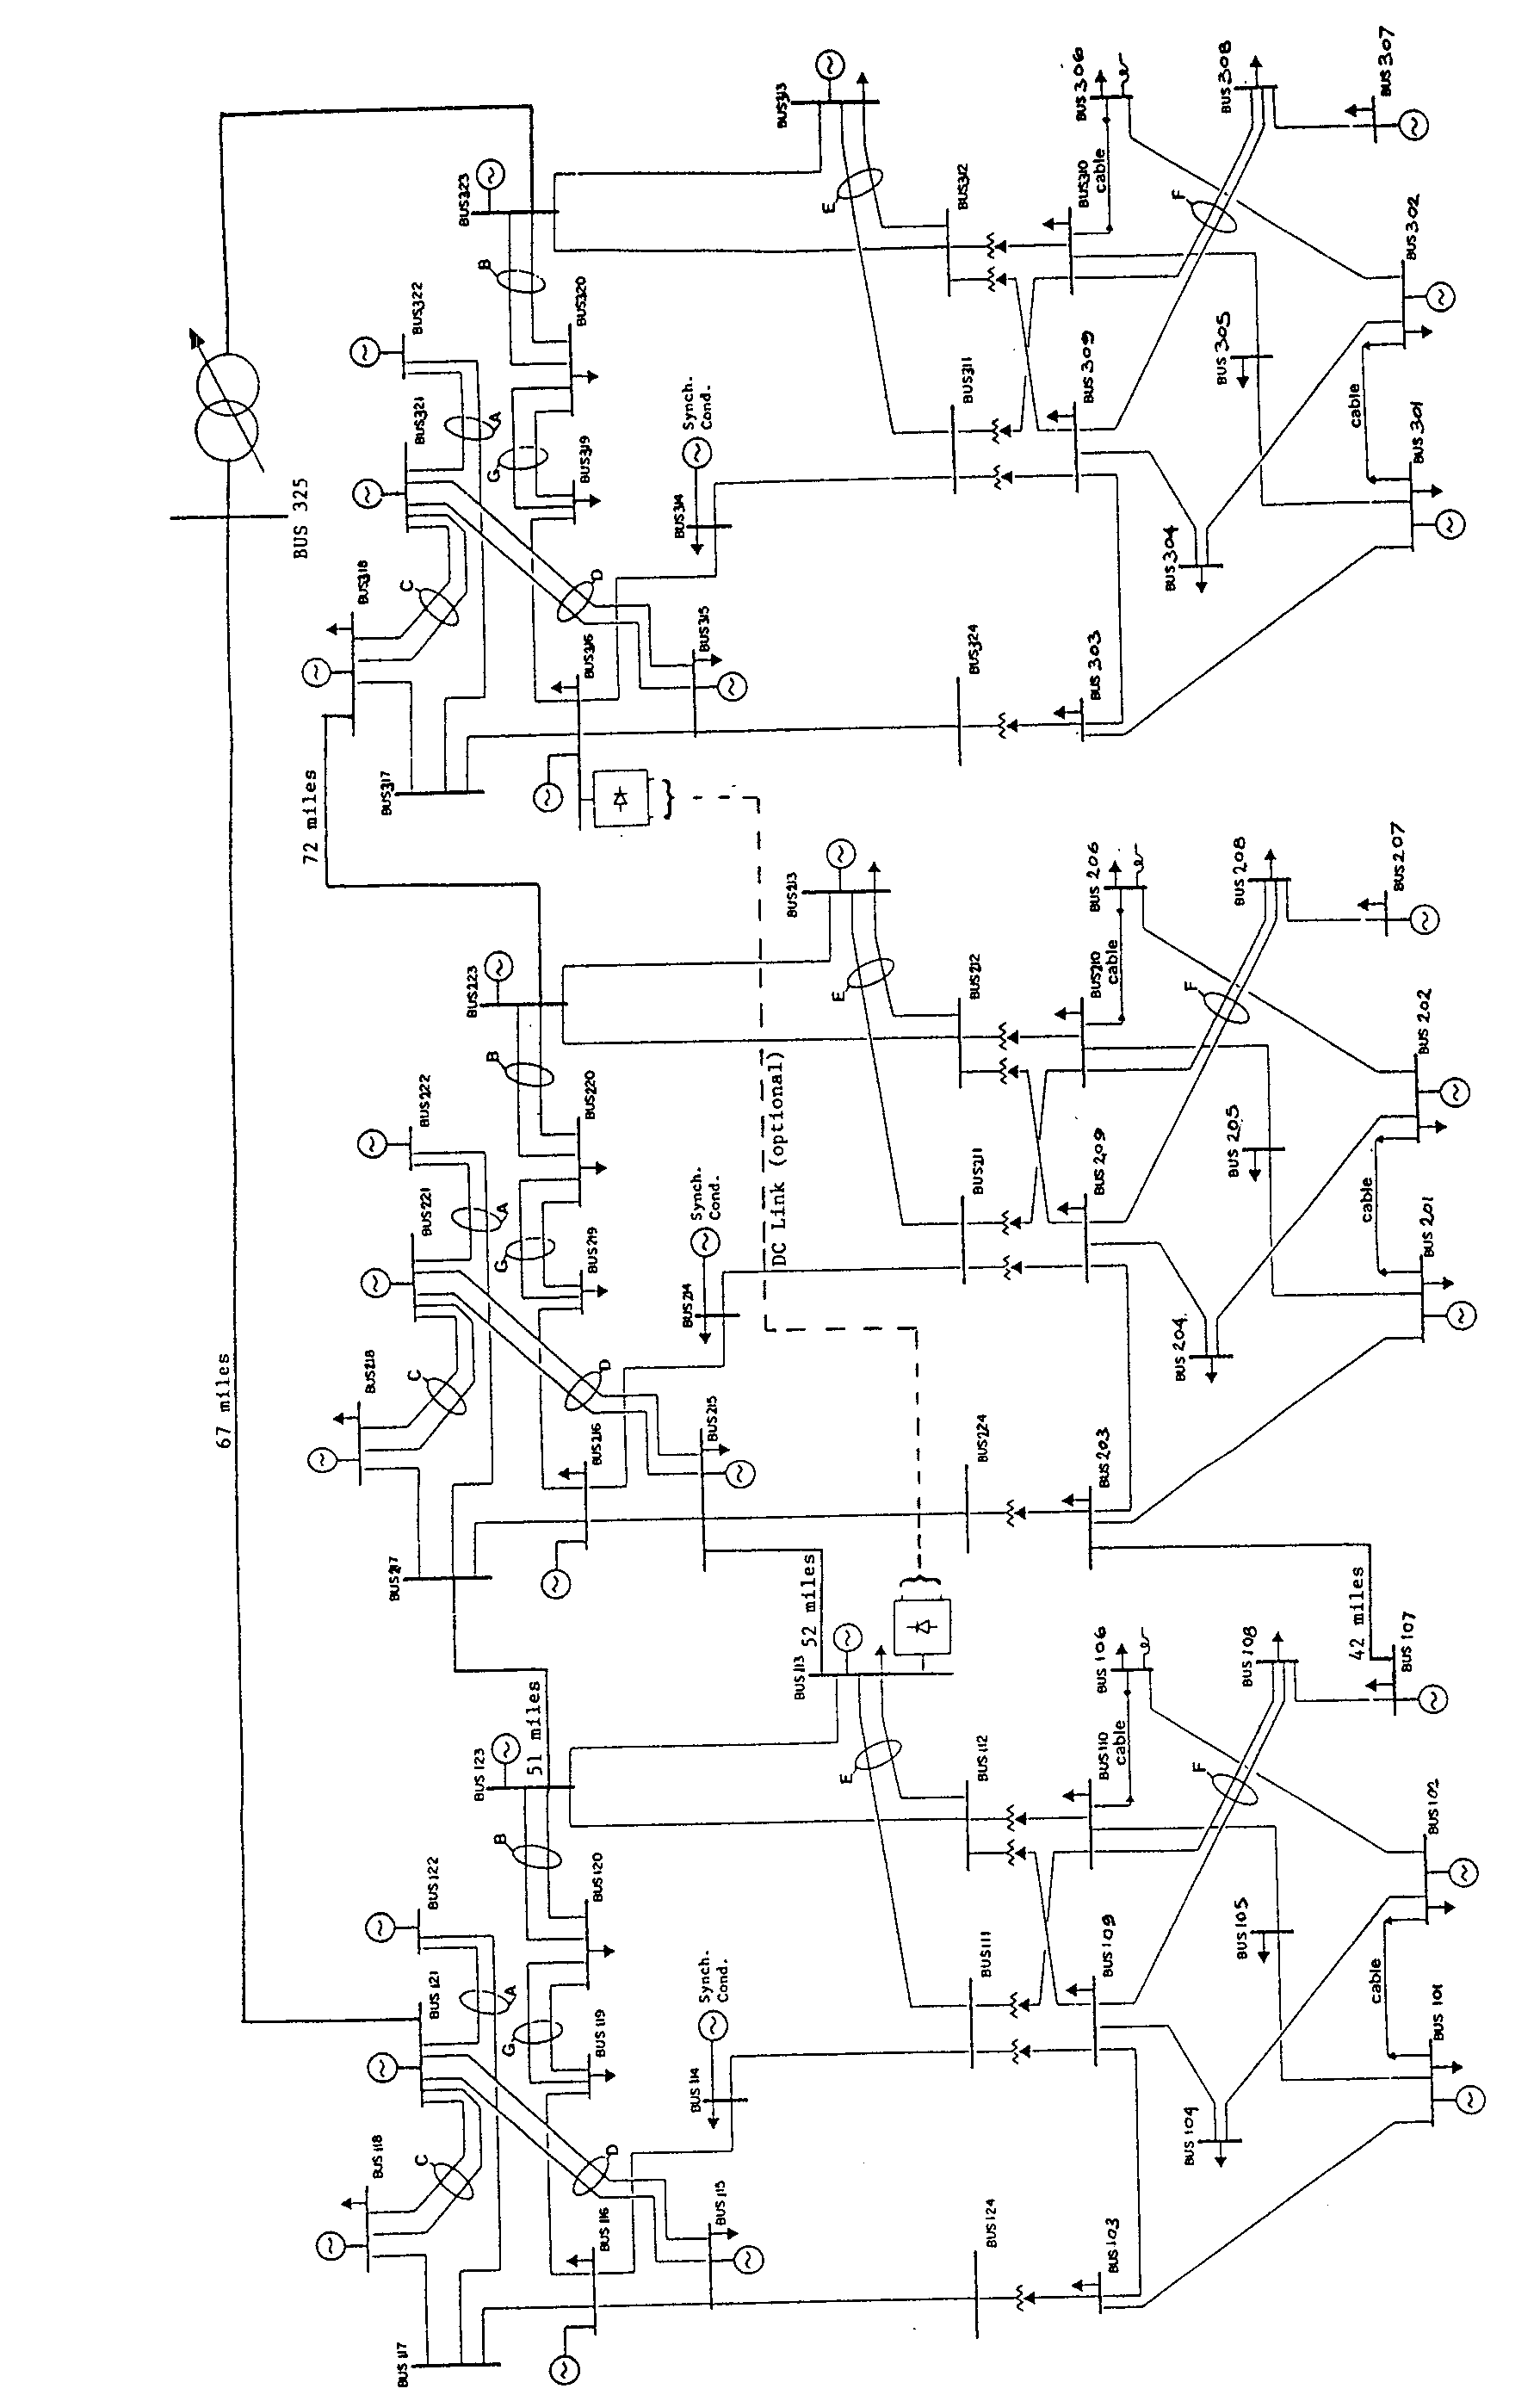
\includegraphics[width=\textwidth,height=\textheight,keepaspectratio]{ieeetopology.png}
  \caption{RTS-96 Topology.}
  \label{fig:ieeetopology}
\end{figure}

The dataset describes a peak load for each bus. The absolute load in every hour is a percentage of the peak load based on 3 components: the week of year, the day of week an the hour of the day. The hourly peak changes according to the season and if it is in a weekend or not. For example, the peak load of bus 101 is 108MW. On 01/07 at 12:00 PM the load is:

\begin{multline}
L_{b = 108} =  (L_{yearweek = 27} = 75.5\%) \times (L_{dayofweek = friday} = 94\%) 
\\ \times (L_{hour= 12 PM} = 93\%) \times 108 = 71.28MW
\end{multline}

Figure \ref{fig:totalSystemLoadJuly} displays the total system load throughout the month of July.

\begin{figure}[H] 
  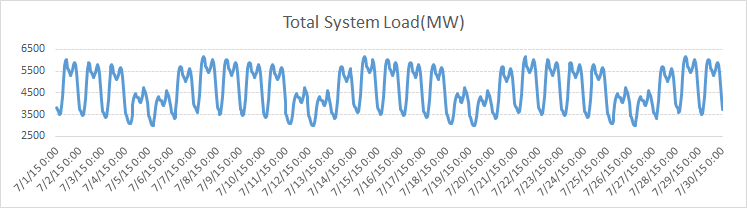
\includegraphics[width=\textwidth,height=\textheight,keepaspectratio]{totalSystemLoadJuly.png}
  \caption{Total System Load (MW) in July 2015.}
  \label{fig:totalSystemLoadJuly}
\end{figure}

To generate instances with sub-hourly load profiles, the load during intra-hour periods is constructed using linear interpolation plus an additional perturbation, which follows a uniform $[-Pr,+Pr]\%$, where $Pr$ is a parameter in the range of [0,100] \%. The objective is to capture the ramping behaviour of NVRE on a sub hourly level. Figure \ref{fig:perturbationDifference} shows a difference between load curves on a 60-minute and 15-minute planning level. 

\begin{figure}[H] 
  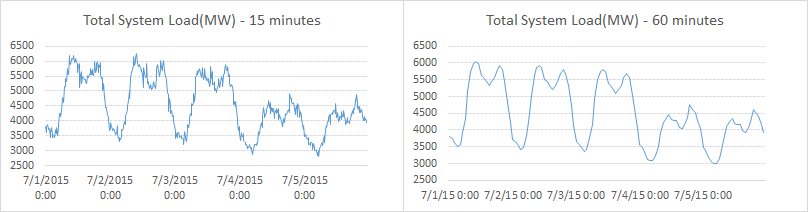
\includegraphics[width=\textwidth,height=\textheight,keepaspectratio]{perturbationDifference.png}
  \caption{System Load (MW) for 5 Days in July With 15- and 60-minute Resolution.}
  \label{fig:perturbationDifference}
\end{figure}

The original RTS-96 system has 87 generators distributed across the test field, with the distribution described in figure \ref{fig:generatorDistribution}. Sync generators are not considered for this study.

\begin{figure}[H] 
  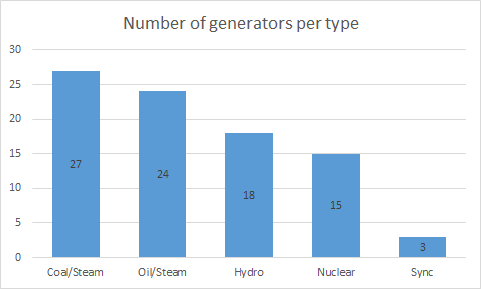
\includegraphics[width=\textwidth,height=\textheight,keepaspectratio]{numberGeneratorsPerType.png}
  \caption{Total Number of Generators per Type.}
  \label{fig:generatorDistribution}
\end{figure}

The total peak load is 8550 MW while the total generation capacity is 9975 MW. 

\subsection{Renewable Generators Data}

Although RTS-96 has most of the necessary data for this project, it does not contain any wind and solar generation information, the two fastest growing renewable sources in the world. This discrepancy is interesting in its own right as it reveals how much technology has changed in the two decades since the RTS-96 data set was published.

Since wind and solar energy are expected to play a prominent role in the future grid (e.g., India has pledged to install 100 GW of solar capacity by 2022 \cite{mitindia}, while Germany has already installed 45 GW of wind capacity, or roughly 25 \% of its total installed capacity\cite{fraunpower}, wind and solar profiles were also included in our test instances. Historical data for both sources was taken from the website of the Electric Reliability Council of Texas (ERCOT), the independent system operator that manages the flow of electric grid for the vast majority of Texas.  

The wind and solar profiles define the generation capacity for these renewable resources in a full year, and it is based on historical availability from the last 5 years in Texas. The geographic renewable potential in Texas were considered for each bus in the system, both for solar and wind generators.

\newpage
\subsubsection{Wind Profile}


Figure \ref{fig:texasWindProfile}, adapted from \cite{texasWindProfile} shows the Texas Annual Average Wind speed and the relative geographic positions of RTS-96 buses \cite{wongieee}. The flat northern border is known as the "panhandle" because the state of Oklahoma, north of Texas, is shaped like a pan. The handle of this pan is where most of the wind potential resides. As a result, most of the new generators are being installed in northwest \cite{texasWindProfile}.

\begin{figure}[H] 
  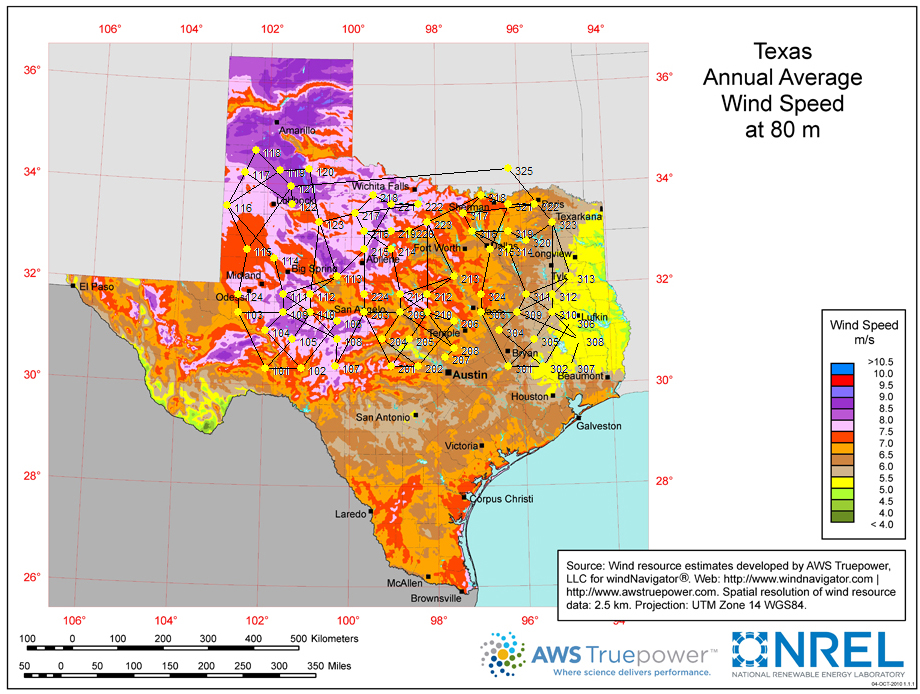
\includegraphics[width=\textwidth,keepaspectratio]{texasWindProfileWithBuses.png}
  \caption{Wind Potential for Texas with RTS-96 Bus Locations.}
  \label{fig:texasWindProfile}
\end{figure}


To build the wind potential, each bus was associated with a Texas city or region along with the average historical wind generation for the past 5 years. The studied data is freely shared by ERCOT \cite{ercotGenerationWind}. Therefore each location has a wind potential on an hourly level throughout an entire year. In sub-hourly levels the availability follows the interpolation between the hours followed by a uniform perturbation, using the same logic as with load. That said, the real generation for any wind generator is a factor of the percentage of the nameplate capacity followed by the profile where it is located. Figure \ref{fig:windProfileBus122January} shows the wind profile for the bus 122 in the month of January.

\begin{figure}[H] 
  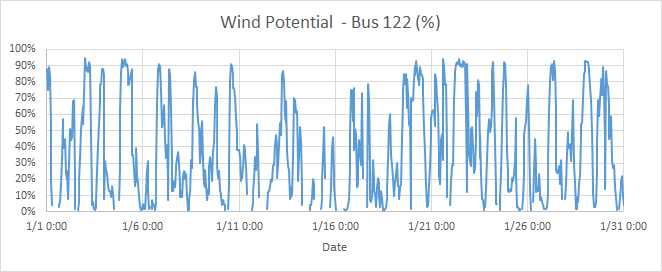
\includegraphics[width=\textwidth,keepaspectratio]{windPotentialBus122.png}
  \caption{Wind Profile for Bus 122 in January.}
  \label{fig:windProfileBus122January}
\end{figure}

\newpage
\subsubsection{Solar Profile}

Figure \ref{fig:texasSolarProfile}, adapted from \cite{texasSolarProfile}, displays the NREL's solar incidence report in the state of Texas and the relative geographic positions of RTS-96 buses. 

\begin{figure}[H] 
	\begin{center}
		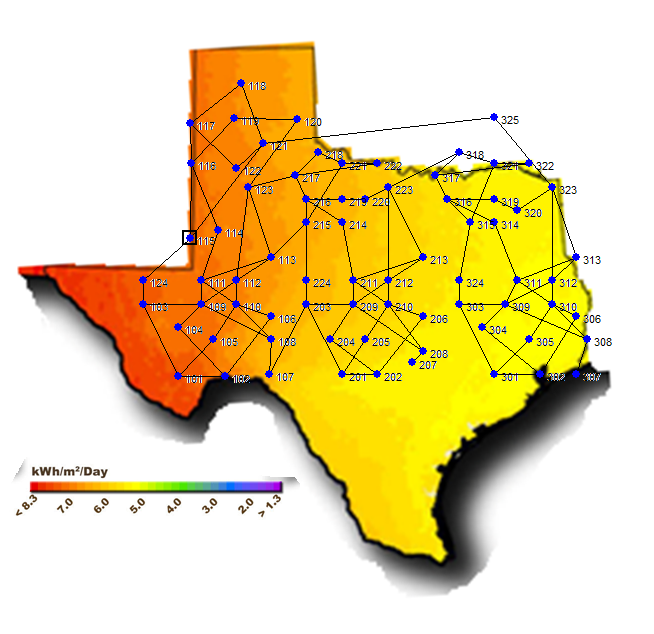
\includegraphics[width=0.6\textwidth,height=\textheight,keepaspectratio]{texasSolarProfileWithBuses.png}
	  	\caption{Solar Potential for Texas with RTS-96 Bus Locations.}	  		\label{fig:texasSolarProfile}
	\end{center}
\end{figure}


It is important to notice that the highest incidence profile in the state of Texas is located in the west, followed by the northeast and center. The solar profile analysis follows the same logic developed in the wind case. However, only buses located in the mentioned area had their profiles built. As an example, the solar profile for bus 112 (in far northeast of Texas) on January is shown in figure \ref{fig:solarProfileBus112January}.

\begin{figure}[H] 
	\begin{center}
		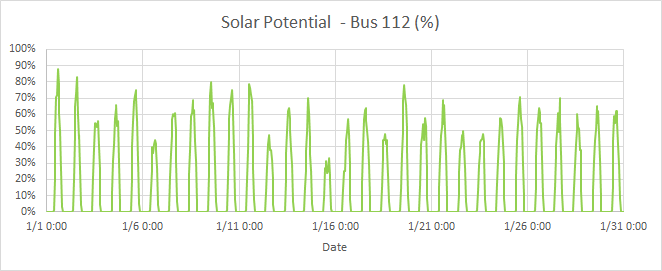
\includegraphics[width=0.8\textwidth,keepaspectratio]{solarPotentialBus112.png}
	  	\caption{Solar Profile for Bus 112 in January.}
     	\label{fig:solarProfileBus112January}
	\end{center}
\end{figure}


\subsection{Costs}

For our models, the costs were developed based on the RTS-96 data and some benchmark values widely used in the industry for power generation studies. There are two type of costs associated with generation:

\begin{itemize}
\item Generation Cost ($\$/MW$): Cost to generate 1MW of a specific unit group.
\item Start-up Cost ($\$/MW$): Cost to change the state of a specific generator type from off to on.
\end{itemize}

\subsection{Scenarios Description} \label{section:ScenarioDesc}

This project covered 3 different generator scenarios in the same load profile. The distribution is adapted from \citeauthor{shavel} \cite{shavel}, that describes the technical and economical potentials of exploring natural gas and VRE in the state of Texas \cite{shavel}. 

\subsubsection{Scenario 1: Reference}

This scenario captures the existing ERCOT capacity mix. 88\% of generation comes from non-renewable energy sources. The remaining capacity is filled by wind generators, located in the buses that have the Texas Northwest's wind potential (Buses 111-124).

\subsubsection{Scenario 2: Stronger Federal Carbon Rule}

Scenario 2 is built based on column "2032 Total" of table IV-10 in \cite{shavel}. This scenario is described as follows:

\begin{quotation}
"Our scenario with a strong federal carbon rule requires existing coal plants to capture and sequester 90\% of their CO2 output.(...)
As one would expect, this case shows that most of the ERCOT coal plant fleet retires in 2025, the year we assume the carbon rule goes into effect. At this point, 16 GW of coal capacity providing more than 30\% of all ERCOT energy rapidly shifts to gas and renewable supply sources: 6 GW of new CC capacity and 3 GW of new wind capacity. In the next several years, another 3 GW of CC capacity is added, along with another 19 GW of wind. Solar becomes rapidly cost-effective in this scenario and quickly rises to over 8 GW installed by 2029. For the remainder of the scenario horizon, all additional load growth is met by solar and wind additions.”
\end{quotation}

In essence, 44\% of the generation is provided by natural gases, followed by 42\% of NVRE and 14\% of other sources. Most of the wind generators are located at buses 111-124, with some in 211-224. Solar generators are at buses 101-110.


\subsubsection{Scenario 3: "Almost Green World"}

This scenario is an extreme case of Scenario 2. All coal, nuclear and oil/steam generators have been retired and are no longer a part of the system. The grid runs entirely on wind and solar, with advanced natural gas combined cycle generators used primarily for ramping, flexibiliy and backup, i.e, to complete the demand when there is not enough wind and solar to fulfil the load. Wind and solar generators are located throughout the map, following the concentration based on wind and solar profiles from figures \ref{fig:texasSolarProfile} and \ref{fig:texasWindProfile}.

\subsubsection{Scenario 4: "Green World"}

In this scenario all the natural gases are replaced by battery storage. The generation is 100\% provided by wind and solar generators, with nameplate capacity bigger than Scenario 3. To mitigate the transmission generation limits, wind generators are located all over the field, while solar generators are still located in north east. There is no decision to turn on and off any generator, and the main decision is only how the storage behaviours in order to minimize under generation.

\subsubsection{Generation per Scenario}

The nameplate capacity of the base case scenario described by \citeauthor{shavel} \cite{shavel} is 82,949 MW, where for RTS-96 is close to 10,000 MW. Therefore all absolute generator type capacities were adapted to the new baseline and the rates by type were mantained. The result is in Table \ref{table:ScenarioDataDescription}.

\begin{table}[H]
\centering
\caption{Capacity of Each Generator Type Expressed in MW as a Percentage of Total Capacity in the 4 Scenarios.}
\begin{tabular}{|lllllll|l|l|}
\hline
               & \multicolumn{2}{l}{\textbf{Scenario 1}} & \multicolumn{2}{l}{\textbf{Scenario 2}} & \multicolumn{2}{l|}{\textbf{Scenario 3}} & \multicolumn{2}{l|}{\textbf{Scenario 4}} \\ \hline
               & \textbf{MW}         & \textbf{\%}       & \textbf{MW}         & \textbf{\%}       & \textbf{MW}          & \textbf{\%}       & \textbf{MW}          & \textbf{\%}       \\ \hline
Nuclear        & 660                 & 6                 & 440                 & 4                 & 0                    & 0                 & 0                    & 0                 \\ \hline
Coal           & 2530                & 23                & 220                 & 2                 & 0                    & 0                 & 0                    & 0                 \\ \hline
Oil/Gas        & 1650                & 15                & 880                 & 8                 & 0                    & 0                 & 0                    & 0                 \\ \hline
NGCC           & 4180                & 38                & 4400                & 40                & 2287                 & 21                & 0                    & 0                 \\ \hline
NGTC           & 2090                & 6                 & 440                 & 4                 & 404                  & 3                 & 0                    & 0                 \\ \hline
Wind           & 660                 & 12                & 3630                & 33                & 7934                 & 60                & 8000                 & 61                \\ \hline
Solar          & 1320                & 0                 & 900                 & 9                 & 2824                 & 16                & 5452                 & 59                \\ \hline
\textbf{Total} & \textbf{11000}      & \textbf{100}      & \textbf{11000}      & \textbf{100}      & \textbf{13452}       & \textbf{100}      & \textbf{17900}       & \textbf{100}      \\ \hline
\end{tabular}
\label{table:ScenarioDataDescription}
\end{table}


\section{Models}

This section describes the Unit Commitment and Economic Dispatch models used in this project

\subsection{Indices and Sets}

\begin{tabular}{ll}

$g \in \mc{G} $& Set of generators\\
$b \in \mc{B} $& Set of buses\\
$sd \in \mc{SD} $& Set of storage devices\\
$g \in \mc{G}^{NR} $& Subset of non-renewable generators\\
$g \in \mc{G}^{R} $& Subset of renewable generators \\
$gt \in \mc{GT} $& Set of generator types \\
$u \in \mc{U} $& Set of unit groups \\
$l \in \mc{L} $& Set of transmission lines \\
$rr \in \mc{RR} $& Set of reserve requirements \\
$rp \in \mc{RP} $& Set of reserve products \\
$t \in \mc{T} $& Set of time periods \\
$g \in \mc{G^{b}} $& Set of generators in each bus b \\


\end{tabular}

\newpage
\subsection{Parameters}

\begin{tabular}{ll}

$D_{b,t} $& Load at bus $b$ in time $t$ \\
$C_{g} $& Generation cost for generator g (\$ / MW) $t$ \\
$S_{g} $& Start-up cost for generator g \\
$R^{up}_{g} $& Ramp up limit for generator g \\
$R^{down}_{g} $& Ramp down limit for generator g \\
$G^{max}_{g} $& Maximum generation capacity for generator g \\
$G^{min}_{g} $& Minimum generation capacity for generator g \\
$T^{min}_{l} $& Minimum transmission of transmission line l \\
$T^{max}_{l} $& Maximum transmission of transmission line l \\
$P^{R}_{g,t} $& Power generation of renewable generator g in time t\\
$U^{up}_{g} $& Minimum uptime of generator g (hours)\\
$U^{down}_{g} $& Minimum downtime of generator g (hours)\\
$ST^{max}_{sd} $& Maximum storage capacity of storage device sd (MW)\\
$ST^{ramp}_{sd} $& Maximum storage capacity of storage device sd (MW)\\

\end{tabular}



\subsection{Variables}

\begin{tabular}{ll}

$P^{NR}_{g,t} $& Power generation of non-renewable generator g in time t (MW)\\
$T_{i,j,t} $& Power transmitted from bus i to bus j in time t (MW)\\
$T^{loss}_{i,j,t} $& Power loss in transmission from bus i to bus j in time t (MW)\\
$S_{g,t} $& On/off status of generator g at time n\\
$S^{on}_{g,t} $& Start-up status of generator g at time n\\
$S^{off}_{g,t} $& Shut-down status of generator g at time n\\
$V^{-}_{b,t} $& Under generation slack variable at each bus b in time t\\
$V^{+}_{b,t} $& Over generation slack variable at each bus b in time t\\
$ST^{max}_{sd,t} $& Amount of energy stored in storage device sd in time t\\
$ST^{charge}_{sd,t} $& Amount of energy charged in device sd in time t\\
$ST^{discharge}_{sd,t} $& Amount of energy discharged in device sd in time t\\

\end{tabular}

\subsection{Models}
The Economic Dispatch model satisfies the load and transmission requirements at a minimum cost, following operational requirements such as generation, transmission and ramp limits. In this model, we assume that the commitment decisions have been already made. The main objective function of the studied models is to minimize operational costs over the planning horizon, including fuel, start-up, storage and other variable costs.
we

The types of constraints that manage the optimal dispatching are:

\begin{itemize}
\item \textbf{Load Constraints:} For each time period, the amount of power produced and discharge from storage should be equal to the total load and amount charged into a storage. Alternatively, in a node, this equation also considers the inbound and outbound power transmitted.
\item \textbf{Ramping Constraints:}  Each generator has technical limitations that limits the amount of increase and decrease from one period to the next. This is especially important when there are considerable load and VRE fluctuations in consecutive periods.
\item \textbf{Generator Limit Constraints:} When turned on, each generator must produce within a minimum and maximum power limit, under normal operating conditions.
\item \textbf{Transmission Constraints:} Transfer of power between buses is bounded by the nominal power capacity of the transmission line
\item \textbf{Reserve Constraints:} Each non-renewable generator must produce an ammount of reserve to satisfy operational and reliability parameters.
\item \textbf{Storage Constraints:} As well as generators, the charging and discharging rates in storage devices also have technological limits, like total capacity and ramp rates.


\end{itemize}

\subsubsection{Simple Economic Dispatch Model}

\begin{subequations}\label{model:simple_ED}
\begin{alignat}{4}
\min ~~& \sum_{t \in T}\sum_{g \in G^{NR}} P^{NR}_{g,t} C_{g} + \sum_{t \in T}\sum_{b \in B} V^{-}_{b,t} + \sum_{t \in T}\sum_{b \in B} V^{+}_{b,t} \label{eq:ObjectiveFunction} \\
s.t. ~~~& \sum_{t \in T} P^{NR}_{g,t} + \sum_{t \in T} P^{R}_{g,t} + \sum_{t \in T}V^{-}_{b,t} = \sum_{t \in T} D_{b,t}  + \sum_{t \in T}V^{+}_{b,t}  &~& \forall t \in T  \label{eq:loadBalanceConstraint} \\
& P^{NR}_{g,t} - P^{NR}_{g,t - 1} \leq R^{up}_{g} &~& \forall t \in T, g \in \mc{G}^{NR}\label{eq:rampUpRateConstraint} \\
& P^{NR}_{g,t -1 } - P^{NR}_{g,t} \leq R^{down}_{g} &~& \forall t \in T, g \in \mc{G}^{NR}\label{eq:rampDownRateConstraint} \\
& G^{min}_{g}\leq P^{NR}_{g,t} \leq G^{max}_{g} &~& \forall t \in T, g \in \mc{G}^{NR}\label{eq:generationBounds}
\end{alignat} 
\end{subequations}

The constraint \ref{eq:loadBalanceConstraint} states the energy balance in every time. The constraints \ref{eq:rampDownRateConstraint} and \ref{eq:rampUpRateConstraint} state that every generator has to obey the ramp limits. The constraint \ref{eq:generationBounds} states the generation limits for each generator. The use of slack variables $V^{-}_{b,t}$ and $V^{+}_{b,t}$ is necessary to always have feasible solutions, and it is important for scenarios where there is a huge renewable penetration, when there's an abrupt variation of generation and there is a over or under generation.   

\subsubsection{Economic Dispatch with Transmission Constraints}

In this case, the model has to consider transmission limits and losses, without transmission costs associated. The objective function \ref{eq:ObjectiveFunction} remains the same, and the constraints \ref{eq:rampUpRateConstraint}, \ref{eq:rampDownRateConstraint} and \ref{eq:generationBounds} are also used. The constraint \ref{eq:loadBalanceConstraint} is replaced by:  

\begin{subequations}\label{model:edTransmissionConstraints}
\begin{alignat}{4}
&\sum_{g \in G^{b}} P^{NR}_{g,t} + \sum_{g \in G^{b}} P^{R}_{g,t} + \sum_{b^{in} \in B} T_{b^{in},b,t} + V^{-}_{b,t} = D_{b,t}  + V^{+}_{b,t} + \sum_{b^{out} \in B} T_{b,b^{out},t}  &~& \forall b \in B, t \in t \label{eq:transmissionBalanceConstraint} \\
& T^{min}_{l} \leq T_{b^{in},b^{out},t} \leq T^{max}_{l}  &~& \forall b \in B, t \in t \label{eq:transmissionLimits}
\end{alignat} 
\end{subequations}

Constraint \ref{eq:transmissionBalanceConstraint} guarantees that the energy balance is always satisfied for every bus: everything that is generated and received from other buses should be equal to what is loaded and sent throughout the line with the respective losses. If this balance is not satisfied then under and over generation slack variables become non-zero. This bounds could also be written according to the difference of phase angles, followed by the susceptance law. In pratice, this would just limit the transmission limits, while adding more complexity to the model. Thus simplifying this law by just limiting the transmission of real power makes it simple and comply with the project objectives.

The constraint \ref{eq:transmissionLimits} defines the transmission bounds for each line.

\subsubsection{Economic Dispatch model with Unit Commitment commitment constraints}
Unit Commitment is the decision that considers the sets of generators that are turned on and off for the planned time horizon. The model includes decision variables to capture ``on'' and ``off'' states for thermal generators in each time period,along with the start-up and shut-down decisions. \citep{palmintier}. The set of constraints are added to the previous model, and the binary nature of the variables makes the problem an MIP, naturally harder to solve computationally \cite{james}. 

\begin{subequations}\label{model:ucConstraints}
\begin{alignat}{4}
& S_{g,t} = S^{on}_{g,t} - S^{off}_{g,t} + S_{g,t}  &~& \forall g \in \mc{G}^{NR} , t \in \mc{T} \label{eq:logconst}\end{alignat} 
\end{subequations}

Constraint \ref{eq:logconst} specifies the logical condition between the binary variables, assuring that a generator can not be on if it was not turned on. The same is valid for turning it off. Constraints \ref{eq:mindownt} and \ref{eq:minupt} forces the generator to follow their minimum downtime and uptime periods when they are turned on or off. 

When there is the decision of turning the generator on or off, ramping and transmitting only apply if the generator is on in a certain time period. Therefore these constraints have the corresponding binary variable, as shown in \ref{model:UC_NewConstraints}. %fix the ramping models

\begin{subequations}\label{model:UC_NewConstraints}
\begin{alignat}{4}
& P^{NR}_{g,t} - P^{NR}_{g,t - 1} \leq R^{up}_{g} S_{g,t} &~& \forall t \in T, g \in \mc{G}^{NR}\label{eq:UCrampUpRateConstraint} \\
& P^{NR}_{g,t -1 } - P^{NR}_{g,t} \leq R^{down}_{g} S_{g,t} &~& \forall t \in T, g \in \mc{G}^{NR}\label{eq:UCrampDownRateConstraint} \\
& G^{min}_{g} S_{g,t}\leq P^{NR}_{g,t} \leq G^{max}_{g} S_{g,t} &~& \forall t \in T, g \in \mc{G}^{NR}\label{eq:UCgenerationBounds}
\end{alignat} 
\end{subequations}

In the Unit Commitment model, each generator must satisfy a minimum period to remain on or off whether  or not there is a state change in a certain period. Down time constraints are useful for maintenance of a generating unit once has been shut down. Uptime constraints are useful to guarantee stability and to reduce equipment degradation. 

\begin{subequations}\label{model:ucMinDownUpConstraints}
\begin{alignat}{4}
& \sum_{i = t}^{t + U^{up}_{g} - 1} S_{g,t} \geq S^{on}_{g,i} U^{up}_{g} &~& \forall g \in \mc{G}^{NR}, t \in \mc{T} \label{eq:mindownt} \\
& \sum_{i = t}^{t + U^{down}_{g} - 1} (1 -S_{g,t}) \geq S^{off}_{g,i} U^{down}_{g} &~& \forall g \in \mc{G}^{NR}, t \in \mc{T} \label{eq:minupt}
\end{alignat} 
\end{subequations}

The ramping constraints \ref{eq:rampUpRateConstraint} and \ref{eq:rampDownRateConstraint} are replaced by constraints \ref{eq:rampUpRateUCConstraint} and \ref{eq:rampDownRateUCConstraint}.

\begin{subequations}
\begin{alignat}{4}
& P^{NR}_{g,t} - P^{NR}_{g,t - 1} \leq R^{up}_{g}(1 - S^{on}_{g,t}) + \max(R^{up}_{g},G^{min}_{g})S^{on}_{g,t} &~& \forall t \in T, g \in \mc{G}^{NR}\label{eq:rampUpRateUCConstraint} \\
& P^{NR}_{g,t -1 } - P^{NR}_{g,t} \leq R^{down}_{g}(1 - S^{off}_{g,t}) + \max(R^{down}_{g},G^{min}_{g})S^{off}_{g,t} &~& \forall t \in T, g \in \mc{G}^{NR}\label{eq:rampDownRateUCConstraint}
\end{alignat} 
\end{subequations}


\subsubsection{Economic Dispatch/Unit Commitment with Storage Constraints}

Under a scenario where renewable resources are the major source of energy, storage devices are crucial to address fluctuations and uncertainties in generation, so they are an important key to keep the system stable \cite{dwyer}. When storage devices are available in the system, their operations are governed by the following constraints:

\begin{subequations}\label{model:storageConstraints}
\begin{alignat}{4}
& ST^{max}_{sd,t} = ST^{max}_{sd,t - 1} + ST^{charge}_{sd,t} - ST^{discharge}_{sd,t}  &~& \forall sd \in SD, t \in t \label{eq:storageLimits} \\
&  -ST^{ramp} \leq (ST^{charge}_{sd,t} - ST^{charge}_{sd,t-1}) + (ST^{discharge}_{sd,t} - ST^{discharge}_{sd,t-1}) \leq ST^{ramp}  &~& \forall sd \in SD, t \in t \label{eq:storageRamping}
\end{alignat} 
\end{subequations}

The load balance constraint at each bus \ref{eq:transmissionBalanceConstraint} also is modified, by incorporating the storage charging and discharging variables for storage devices located at the specific bus, as defined in equation \ref{eq:transmissionBalanceConstraintStorage}

\begin{subequations}
\begin{align}
\begin{split}
\sum_{g \in G^{b}} P^{NR}_{g,t} + \sum_{g \in G^{b}} P^{R}_{g,t} + \sum_{b^{in} \in B} T_{b^{in},b,t} + V^{-}_{b,t}  + ST^{charge}_{sd \in b,t} &
\\ = D_{b,t}  + V^{+}_{b,t} + \sum_{b^{out} \in B} T_{b,b^{out},t} + ST^{discharge}_{sd \in b,t}  & \forall b \in B, t \in t \label{eq:transmissionBalanceConstraintStorage}
\end{split}
\end{align} 
\end{subequations}

In the case where there is no transmission constraints, the storage is incorporating in the general balance constraint \ref{eq:loadBalanceConstraint}

\begin{subequations}
\begin{align}
\begin{split}
\sum_{t \in T} P^{NR}_{g,t} + \sum_{t \in T} P^{R}_{g,t} + \sum_{t \in T}V^{-}_{b,t} + \sum_{sd \in \mc{SD}} ST^{discharge}_{sd,t} &
\\ = \sum_{t \in T} D_{b,t}  + \sum_{t \in T}V^{+}_{b,t} + \sum_{sd \in \mc{SD}} ST^{charge}_{sd,t} & \forall t \in T  \label{eq:loadBalanceConstraintStorage}
\end{split}
\end{align} 
\end{subequations}

It is important to highlight the difference between storage, reserve and slack variables in the power systems planning context.  \citeauthor{rebours} \cite{rebours} defines reserve as the capacity of generating active power that was still not committed yet during each time period, and it is used mainly to regulate the frequency, improve system stability and security and respond to unexpected events. Storage is the capability to retain the excess of power generated that was not used and can be used afterwards, either to respond to a low demand, an unexpected peak or a power outage from other generators. Both reserve and storage plays an important key the more VREs are present in the power system. Slack variables guarantees the optimal solution even in the case where there is an unbalance between demand and generation, and it is also an important parameters of analysis when wind and solar is available. In simple storage models, where storage capacity is considered infinite, slack variables can indicate bottlenecks in the transmission system, either indicating a failure in transmission of excess power from generator to the storage device or the necessary power from the storage device to a specific load. When transmission constraints is neglected, the over generation slack variable $V^{+}_{b,t}$ is not necessary, once every generation excess is stored for future uses.



\section{Assumptions}

The following assumptions were made in the model and data during the research and development process:

\begin{enumerate}
\item The load profile is deterministic. There is no forecast error and no variability in the hourly levels peak. For sub-hourly levels all the analysis were made assuming a $\pm20\%$ of perturbation
\item In the Economic Dispatch model, the generation is upper bounded only. All generators can produce from 0 up to their maximum capacity
\item All generators are assumed to be on and ready to generate according to their ramping policies at time zero.
\item There is no voltage angle constraint in the model.
\item The model covers the DC version of the ED and UC problems, i.e., only active power is the set of study. There is no reactive power in the developed models.
\item A transmission loss of 1 \% per 100 miles is assumed, which is a coarse representation of reality, but can be easily modelled withing a mixed-integer linear program. This percentage was estimated based on the work of \citeauthor{short} \cite{short}.
\item The load profiles for buses are positively correlated, and are ruled by the hour, day of week, season and day of week type (weekend or not).
\item The following costs are not presented in the model: transmission, maintenance and emission.
\item There are no maintenance factors in generators, like MTTR and MTBF, as well as scheduling. All generators are able to produce power 24 hours per day in ED model and if they are turned on in UC. The same assumptions are made to transmission lines.
\item The generation cost is linear per MW.
\item Although the reserve requirements of NVRE is described in this thesis, they are not considered in this work. Therefore there is no reserve requirement and capacity for NVRE.
\item The generation of renewable resources are not in the decision variables. The developed models only decides the generation for non-renewable resources. Therefore the generation is considered a deterministic parameter, not a variable in the model.
\item The load profile is the same for every year.
\item The peak load is constant and deterministic. No stochastic factor is considered in this study.
\item Heath rates are assumed constant as a function of power output.
\item For the storage scenarios, it is assumed unlimited storage capacity. Thus all the over generated power is stored for future uses.
\item The storages are assumed to be 100\% efficient, so everything is stored is instantly available to fulfil the load.
\end{enumerate}

\section{Implementation}


\subsection{Software Selection}

During the briefing process, it was necessary to choose the software platform that matches our project goals, such that it allows the development, run an analysis the project feasible time. 3 options were considered:

\subsubsection{MATPOWER}

MATPOWER is a powerful tool designed to solve AC and DC Power Flow (PF) and Optimal Power Flow (PF) problems. It is an add-on to MATLAB, and is mainly used for education and research, with some small use on industry. \cite{zimmerman} Although \citeauthor{zimmerman} states that is is possible to dispatch the generators on a minimal quadratic or linear cost, it has limitations on committing them, i.e., solving the UC problem in a multi-period environment. MATPOWER is very powerful on a single time period, but it can provide computational challenges for multi-periods on a larger horizon. Therefore we concluded this tool was not appropriate for this project.

\subsubsection{PLEXOS \textregistered }

PLEXOS \textregistered is a commercial tool for power systems planning, widely used in the power industry for energy resources planning and analysis. It provides an academic license, although the process of obtaining one is long. One of reasons for not using it was the commercial nature of the tool, which could lead to challenges in make everything developed in this thesis available to the academic community.  

\subsubsection{AIMMS}


AIMMS is a mathematical programming tool designed to solve optimization problems. It is as powerful as other optimization tools like AMPL and GAMS. Some features include \cite{bisschop}:

\begin{itemize}
\item Easy-to-use design of complex parameters
\item Intuitive representation of calendar and time horizons
\item Set of optimization tools to solve LP, QP, NLP and MINLP problems
\item GUI to build end-user interfaces
\item Open Data Base Connectivity (OBDC) and OLE interfaces, allowing data exchange between most common databases, such as Oracle, SQL Server, etc.
\end{itemize}

Due to the easiness of use, the fact that an academic license provides 100\% of the tool functionality, and the previous experience of the members of this project, AIMMS was chosen as the supporting tool for this work. The software features are described in next section.

\section{Software Features}

This section briefly cover all the screens and features developed in AIMMS for this project.

\subsubsection{Data Import}

The data import section allows the user to import all the data necessary for our model using the AIMMS specific structure for data text exchange. More details on how prepare the data can be found at \cite{bisschop}.

\begin{figure}[H] 
	\begin{center}
		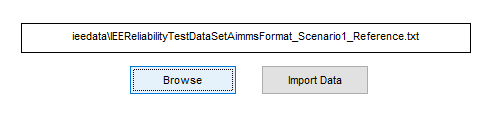
\includegraphics[keepaspectratio]{aimmsScreenImportPage.png}
	  	\caption{Data Import Page in AIMMS.}
     	\label{fig:aimmsScreenImportPage}
	\end{center}
\end{figure}

\newpage
\subsubsection{Data Settings}

After the data has been imported, the user has the chance to add/edit and view some data in an intuitive way. In \textit{Network Page}, it is possible to see the location of buses (in yellow), as well as locations of generators by type. The user can change the list to see whatever type he/she wants. In \textit{Data Buses Page}, it is possible to edit the peak load of each bus in the system. The \textit{Costs Page} has the start-up and variable cost for each generator type and unit group. In \textit{General Data Page} the user can add, edit and remove the main components of the system, i.e., buses, generators and unit groups, as well as changing general configurations, such as horizon dates, granularity and perturbation level for load and wind profiles under a sub-hourly level. 

It is possible also to see the total load over time. In \textit{Generators Specification Page} it is possible to configure the main parameters that define a generator, such as its type, unit group and the bus where it is located. In \textit{Wind and Solar Availability Page} it is possible to view the Wind and Solar profile for the selected bus in the node, as well as locations that have either solar or wind profile mapped (marked with the blue ball). Lastly, the \textit{Summary Page} summarizes the total generation capacity and load, as well as total number of generators and its capacity per generator type.

\newpage
\begin{figure}[H] 
	\begin{center}
		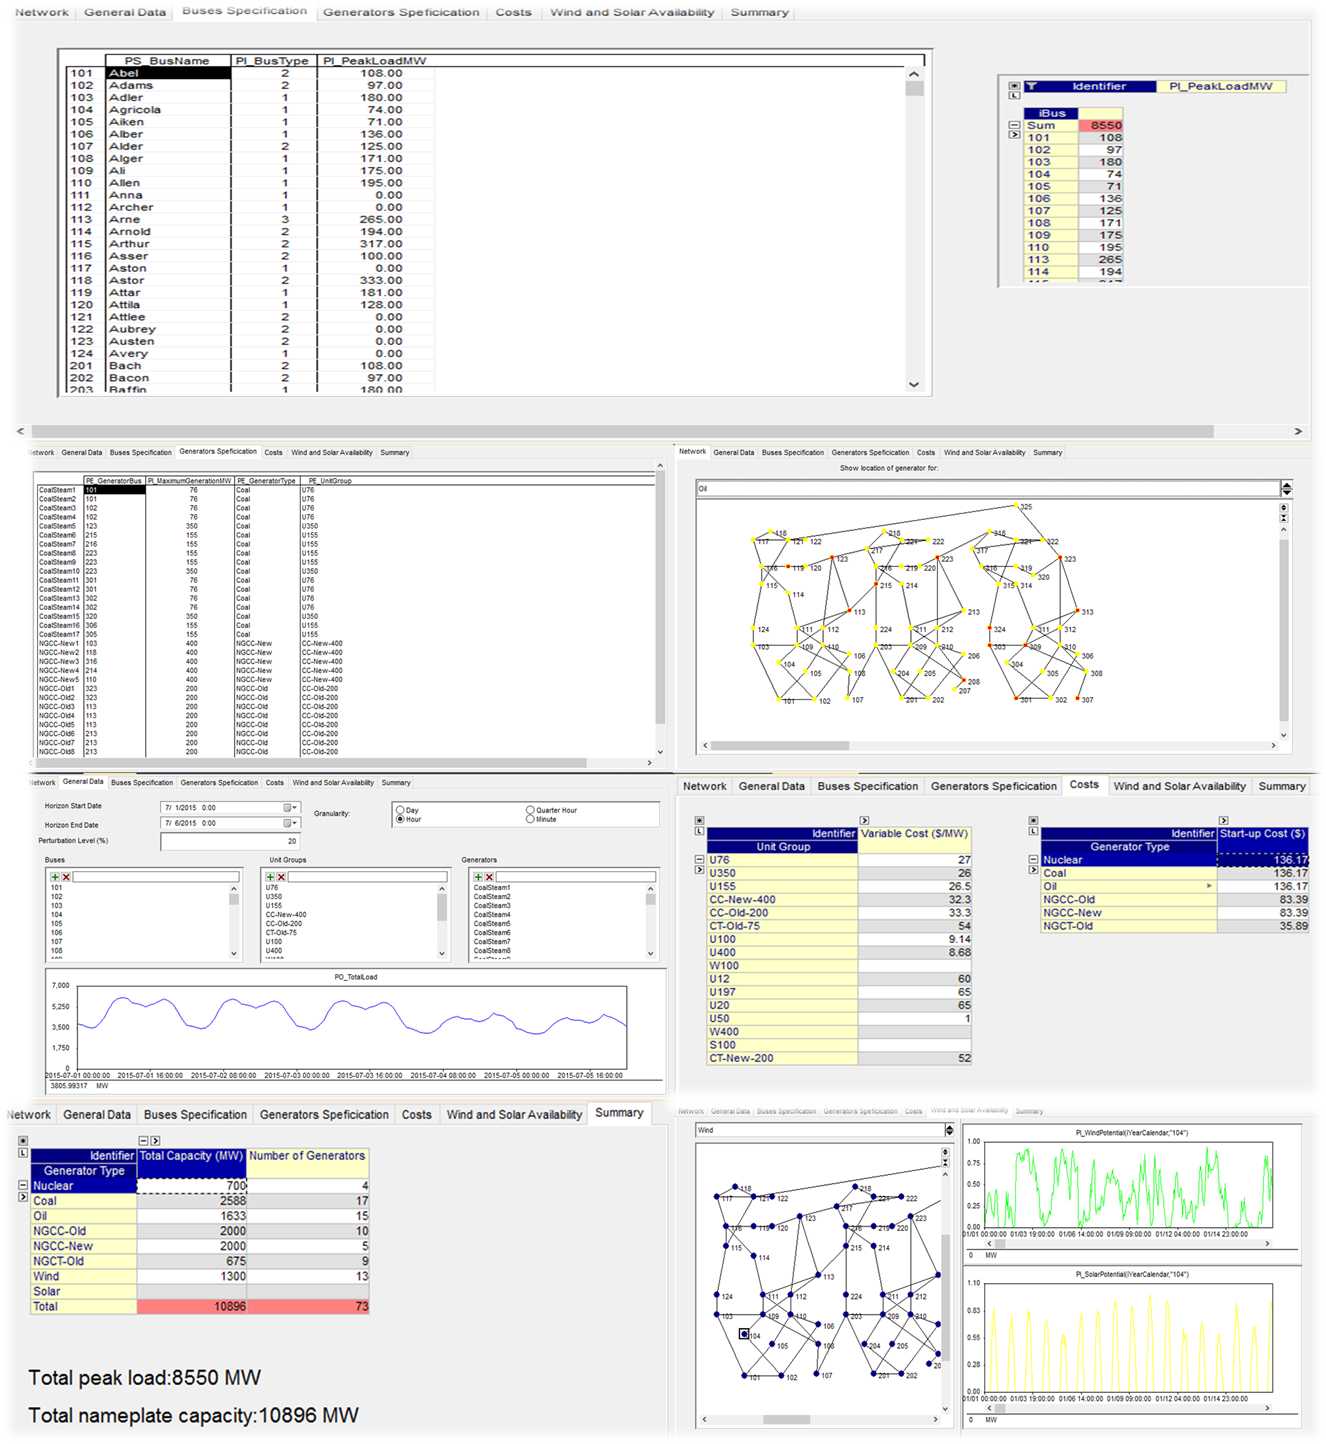
\includegraphics[width=\textwidth,height=\textheight,keepaspectratio]{aimmsDataPages.png}
	  	\caption{Data Section Pages.}
     	\label{fig:dataSectionPages}
	\end{center}
\end{figure}


\subsubsection{Optimization and Results}

The optimization section contains all the required settings to run the optimization, as well as the tables and graphs to analyse the results in an intuitive way. 
The optimization section contains all the required settings to run the optimization, as well as the tables and graphs to analyse the results in an intuitive way. 

The user has the option either to solve the Economic Dispatch or Unit Commitment problems, with or without the following features:

\begin{itemize}
\item Ramping Constraints
\item Transmission Constraints
\item Reserve Constraints
\item Slack Variables
\item Transmission Losses (if "Transmission Constraints" is chosen)
\end{itemize}

In \textit{Demand, Load and Transmission}, it is possible to see, for every bus in every time period, the load, generation and transmission flows in and out. It also is possible to see this same flow in a graphic way in \textit{Transmission Map} section, for each time time period, as well as the location of VRE(in green) and active(red) and inactive(gray) NVRE. The \textit{Average Load Distribution} contains the graph displaying the average load for each generator type within a day, while in \textit{Load Distribution Page} it is possible to see the generation distribution per time period, as well as the total load, being useful to identify over and under generation. The \textit{Power Output Result} details the generation by each generator, in a table. Finally, the \textit{Location Marginal Prices} page contains the Shadow Prices by time period for each location, and it is useful to identify potential investments or bottlenecks.

The \textit{Average Ramping} page is useful to compare the ramping behaviour of the generator sources, expressed as:

\begin{equation}
    AverageRamping_{gt \in \mc{GT}} = \overline{\dfrac{P^{NR}_{g,t} - P^{NR}_{g,t-1}}{G^{max}_{g}}}
\end{equation}

In other words, it expresses the average ramping grouped by each generator type , normalized by its maximum capacity. It avoids the misunderstanding of high-capacity generators being ramped more quickly than the lower ones.

\begin{figure}[H] 
	\begin{center}
		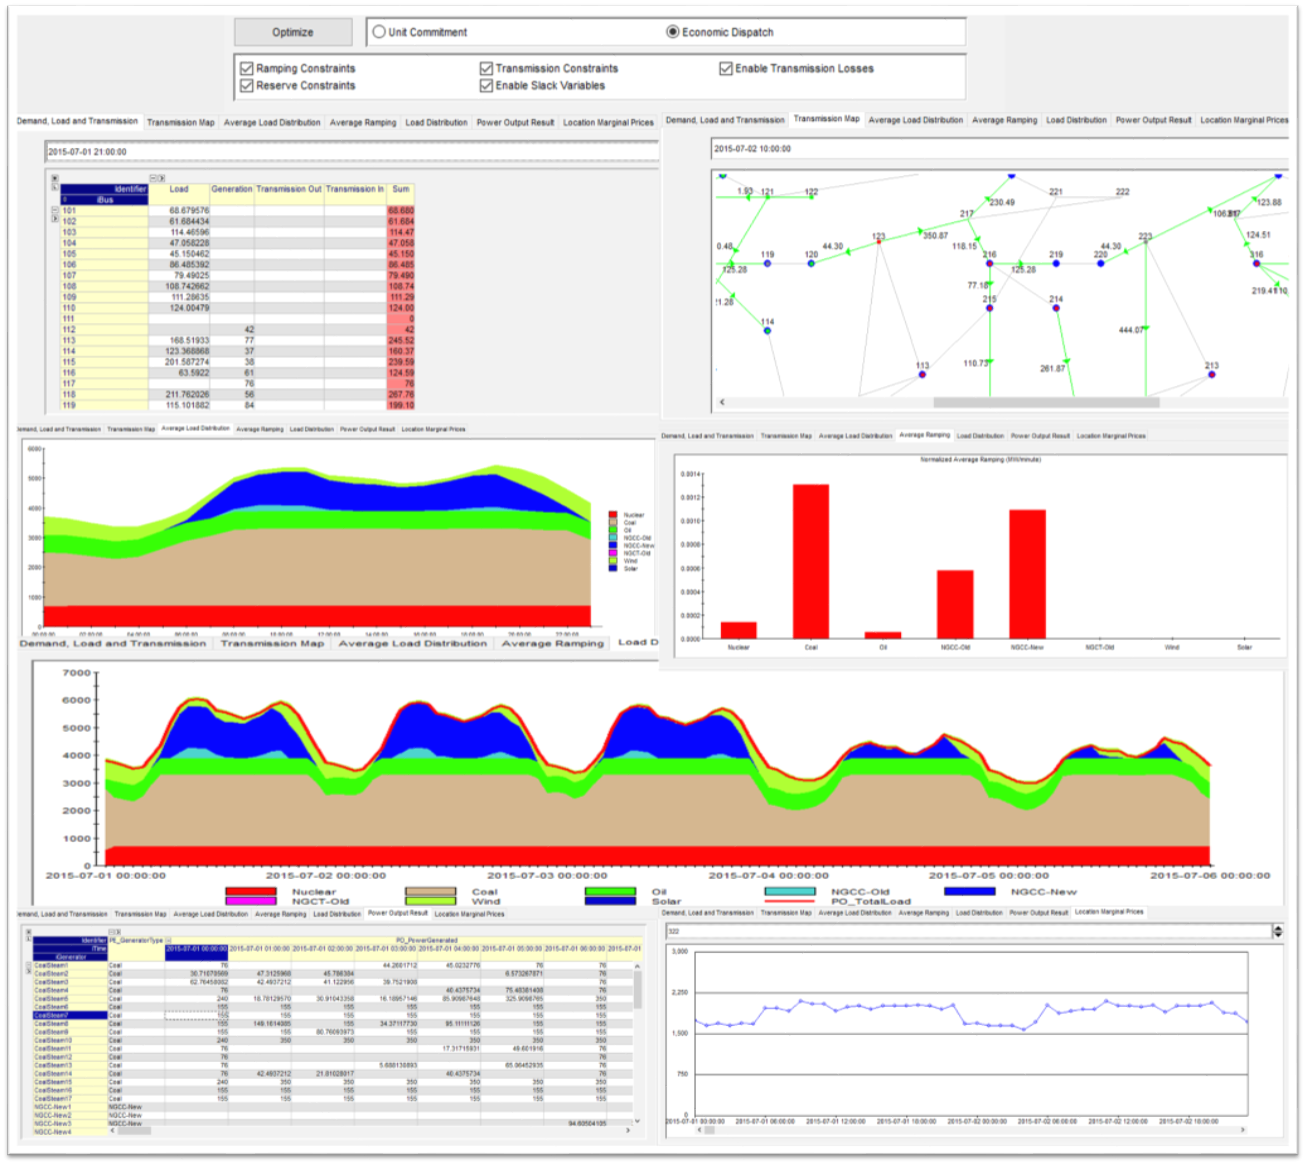
\includegraphics[width=\textwidth,height=\textheight,keepaspectratio]{aimmsOptimizationSectionPages.png}
	  	\caption{Optimization Section Pages.}
     	\label{fig:optimizationSectionPages}
	\end{center}
\end{figure}



\chapter{Analysis}

Our analysis has the primary goal of determining the impact of the following components in the UC and ED models:

\begin{itemize}
\item Time granularity: 1 hour, 15 minutes and 5 minutes.
\item Transmission: with or without transmission constraints.
\item Level of VRE: Scenarios 1, 2 and 3.
\end{itemize}

With all possible combinations of these factors, there are 18 UD and 18 ED data sets to analyse. These are defined as \textit{test cases}. The scenario name format in the graphs and analysis follows the following pattern:
"Scenario Name" \_ "Time Granularity" \_ "Transmission Constraints ON/OFF (TY/TN)" \_ "Model Type (UC/ED)". For example, Scenario2\_15\_TY\_UC test case represents the Unit Commitment model run on a 15-minute level with transmission constraints on in the generator profiles of Scenario 2.

The following metrics are outputs of analysis:

\begin{itemize}
\item Power Output per generation type over time
\item Optimization Parameters
\item Transmission Results
\item Ramping Results
\item Unit Commitment Results
\end{itemize}

All the tests were run on a Intel Core 2 Duo processor with 3.0 GB of RAM memory running under Windows 10 operating system, using CPLEX 12.6.0, executed under AIMMS 4.19.


\section{Power Output per Generation Type}

Figures \ref{fig:powerOutputScenario1}, \ref{fig:powerOutputScenario2} and \ref{fig:powerOutputScenario3} show the power production for each generator type for each model type (UC or ED), granularity (60, 15 and 5 minutes) and transmission constraints on and off. Each combination of these factors are defined as instance. Each figure represents the result for each scenario described in the Data Section. All instances represent the same time period of one week of July, with the same load profile. The generator legend are described at the bottom of the figures, and to make the curves more analysis friendly, all the x-axis were removed. In a general result, for each scenario the instances led to very similar results, with minor particularities, as it will be described by each scenario.

\subsection{Scenario 1}


For scenario 1 the generation profile was the same for nuclear, coal and oil sources for the Economic Dispatch model. When the model is solved with transmission constraints, NGCC-New generators are no longer sufficient to handle the demand at peak load, so they need to be complemented by NGCC-Old ones. The reason for this is that the transmission limits on power transmission, which does not allow NGCC-New generators to fill all the remaining demand at peak, thus NGCC-Old generators must supply it. As for Unit Commitment, different time levels led to minor difference in Oil and NGCC-Old behaviours. Still, the base sources (Nuclear, Coal and Oil) had predominantly the same conduct. These differences are better explored in the section \ref{section:uconoffstatus}.

\begin{figure}[H]
  \centering
	  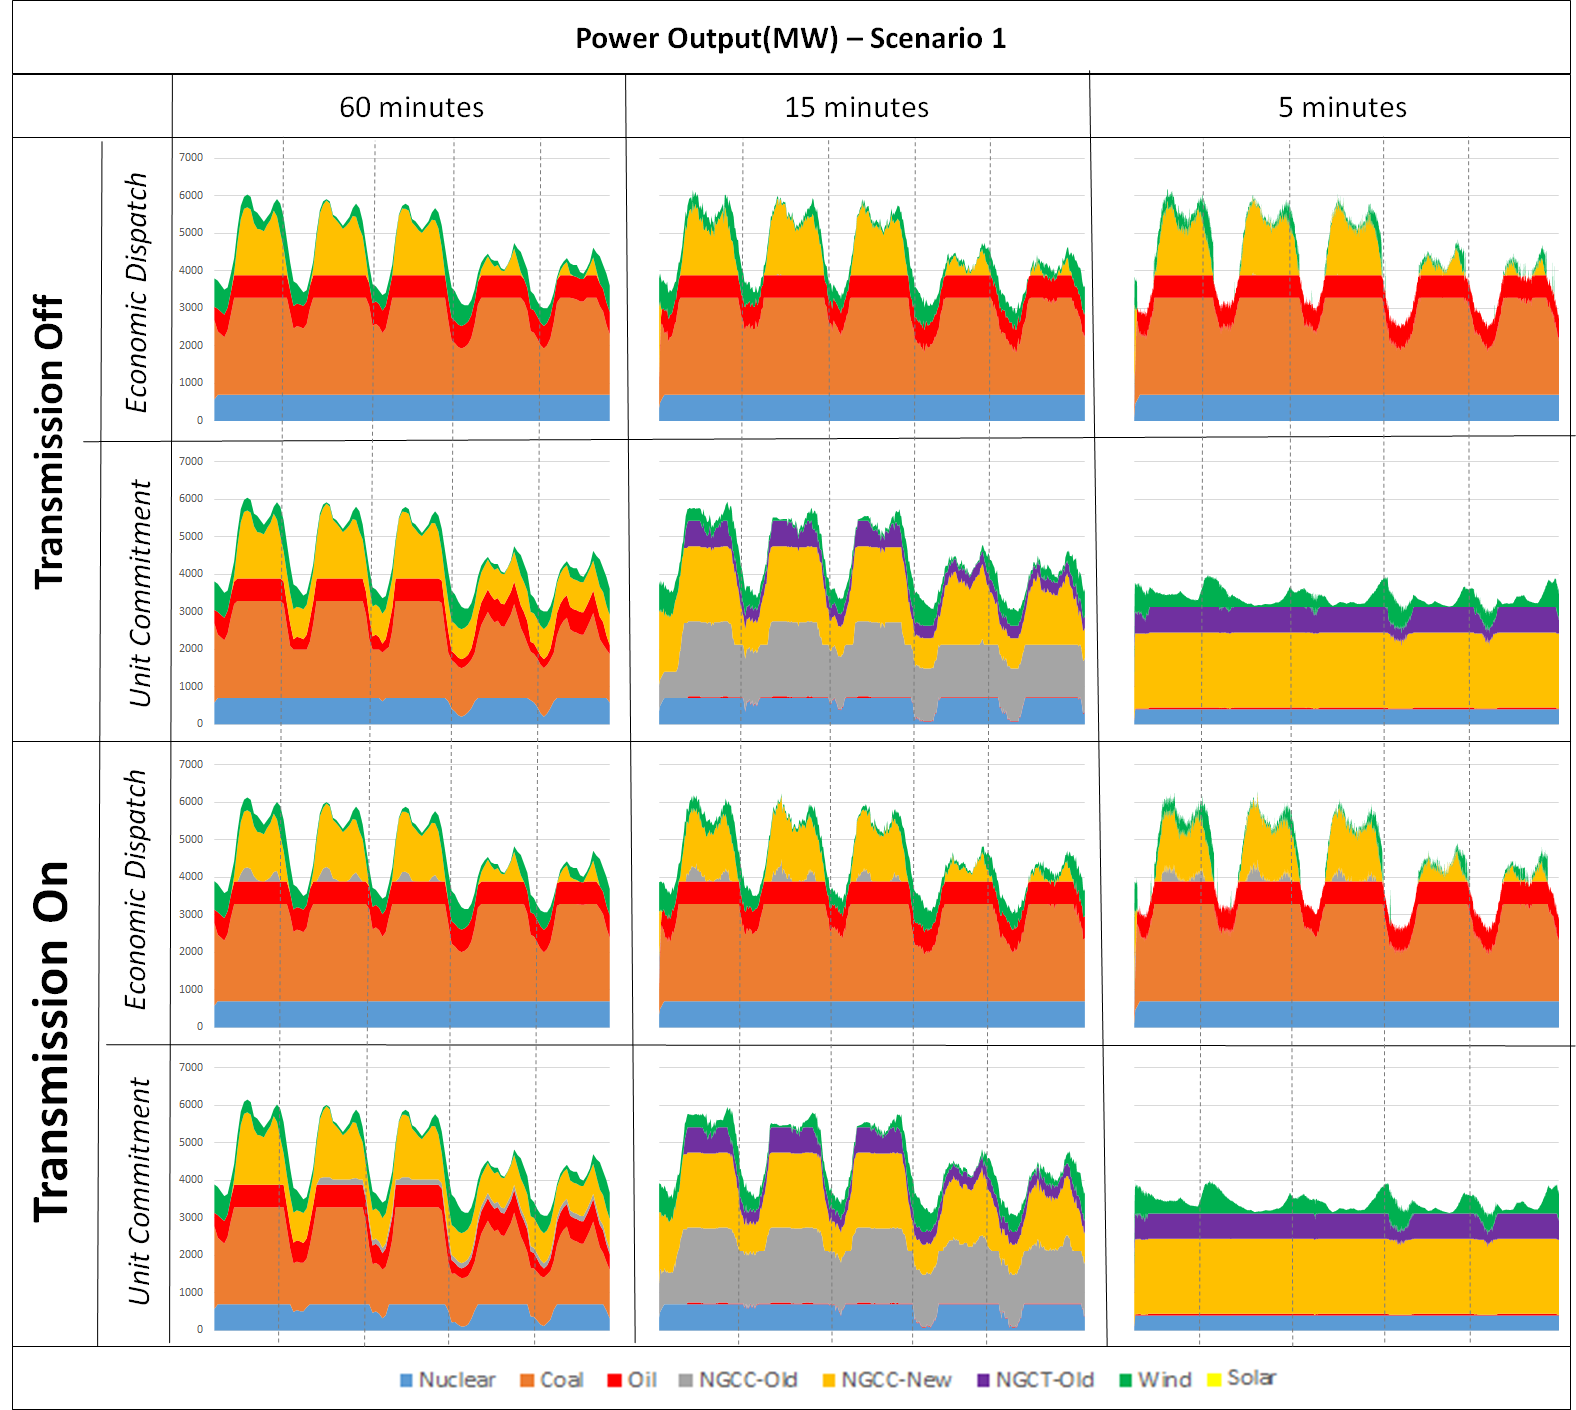
\includegraphics[width=\textwidth,height=\textheight,keepaspectratio]{PowerOutputScenario1.png}
  \caption{Power Output for Scenario 1.}
  \label{fig:powerOutputScenario1}
\end{figure}


\subsection{Scenario 2}

For Scenario 2, in all instances Coal, Oil and Nuclear generators were set to run throughout the whole planning horizon, where NGCC-New generators were chosen to handle peak load and renewable resources variabilities across the time. There are two main differences in the plannings per scenario: in Economic Dispatch models, at the beginning of horizon it is observed a minor ramp of Nuclear, Coal and Oil generators. The deeper the time planning level goes, more was the ramp. After that their generation remain stable during the whole period. In Unit Commitment levels, that does not happen. It was also observed a minor decrease in their generation during a period of low demand and high wind generation on the intance S2-5-TN-UC. This can be explained by the minimum generation levels of NGCC-New generators, so it was more economically beneficial to reduce the generation of cheaper generators then turning off and on some NGCC-New afterwards. However, the same behaviour was not observed on a 60 and 15 minutes level.

%On a 60-minute level, the distribution is almost the same for the Economic Dispatch solutions, but in this case coal and nuclear generators reduce their production when the demand is low and let NGCC-New ones fill the gap. This can lead to increase of maintenance costs because of the ramping behaviour, where in the other hand it strengthen the use of green energy. 

\begin{figure}[H] 
  \centering
	  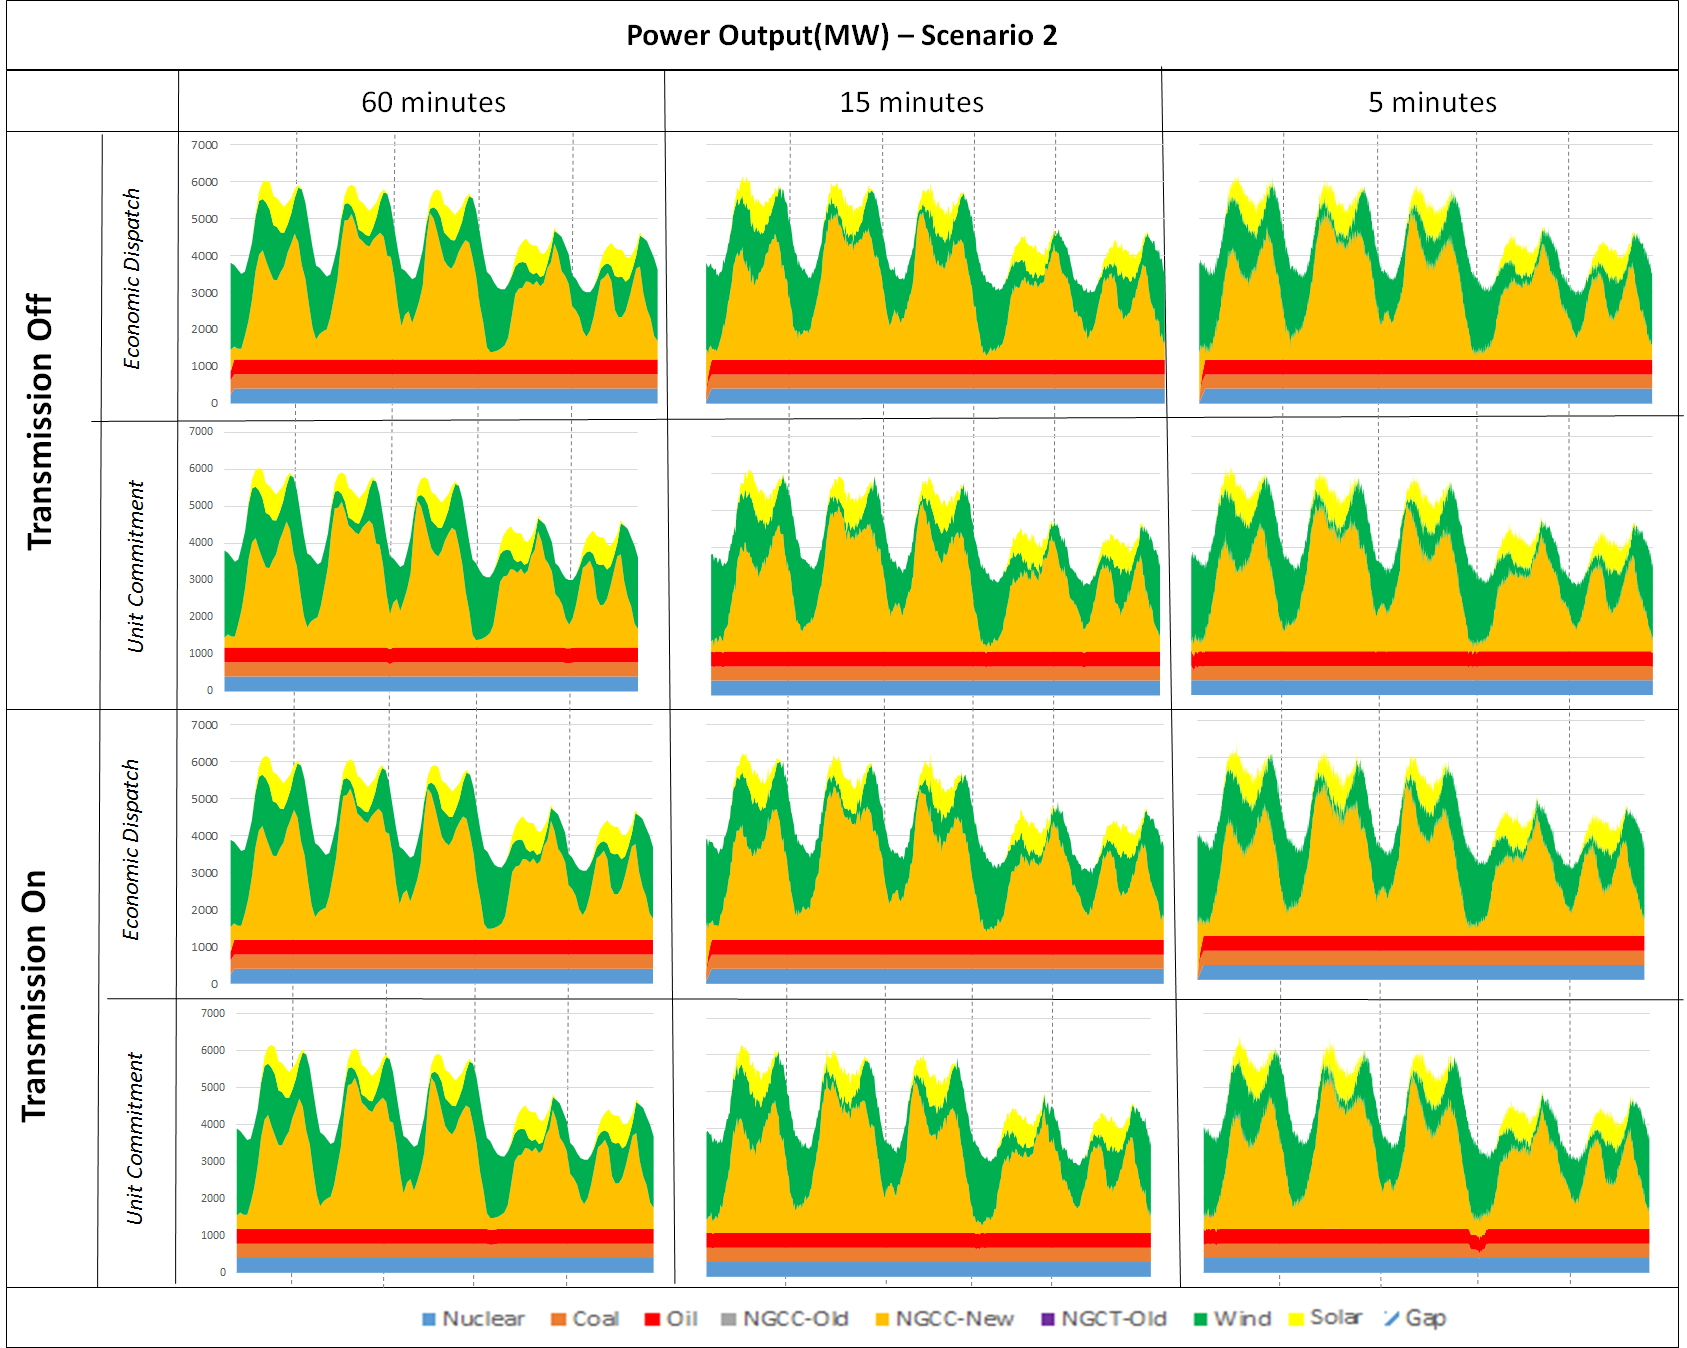
\includegraphics[width=\textwidth,height=\textheight,keepaspectratio]{PowerOutputScenario2.png}
  \caption{Power Output for Scenario 2.}
  \label{fig:powerOutputScenario2}
\end{figure}

\newpage
\subsection{Scenario 3}

\begin{figure}[H] 
  \centering
	  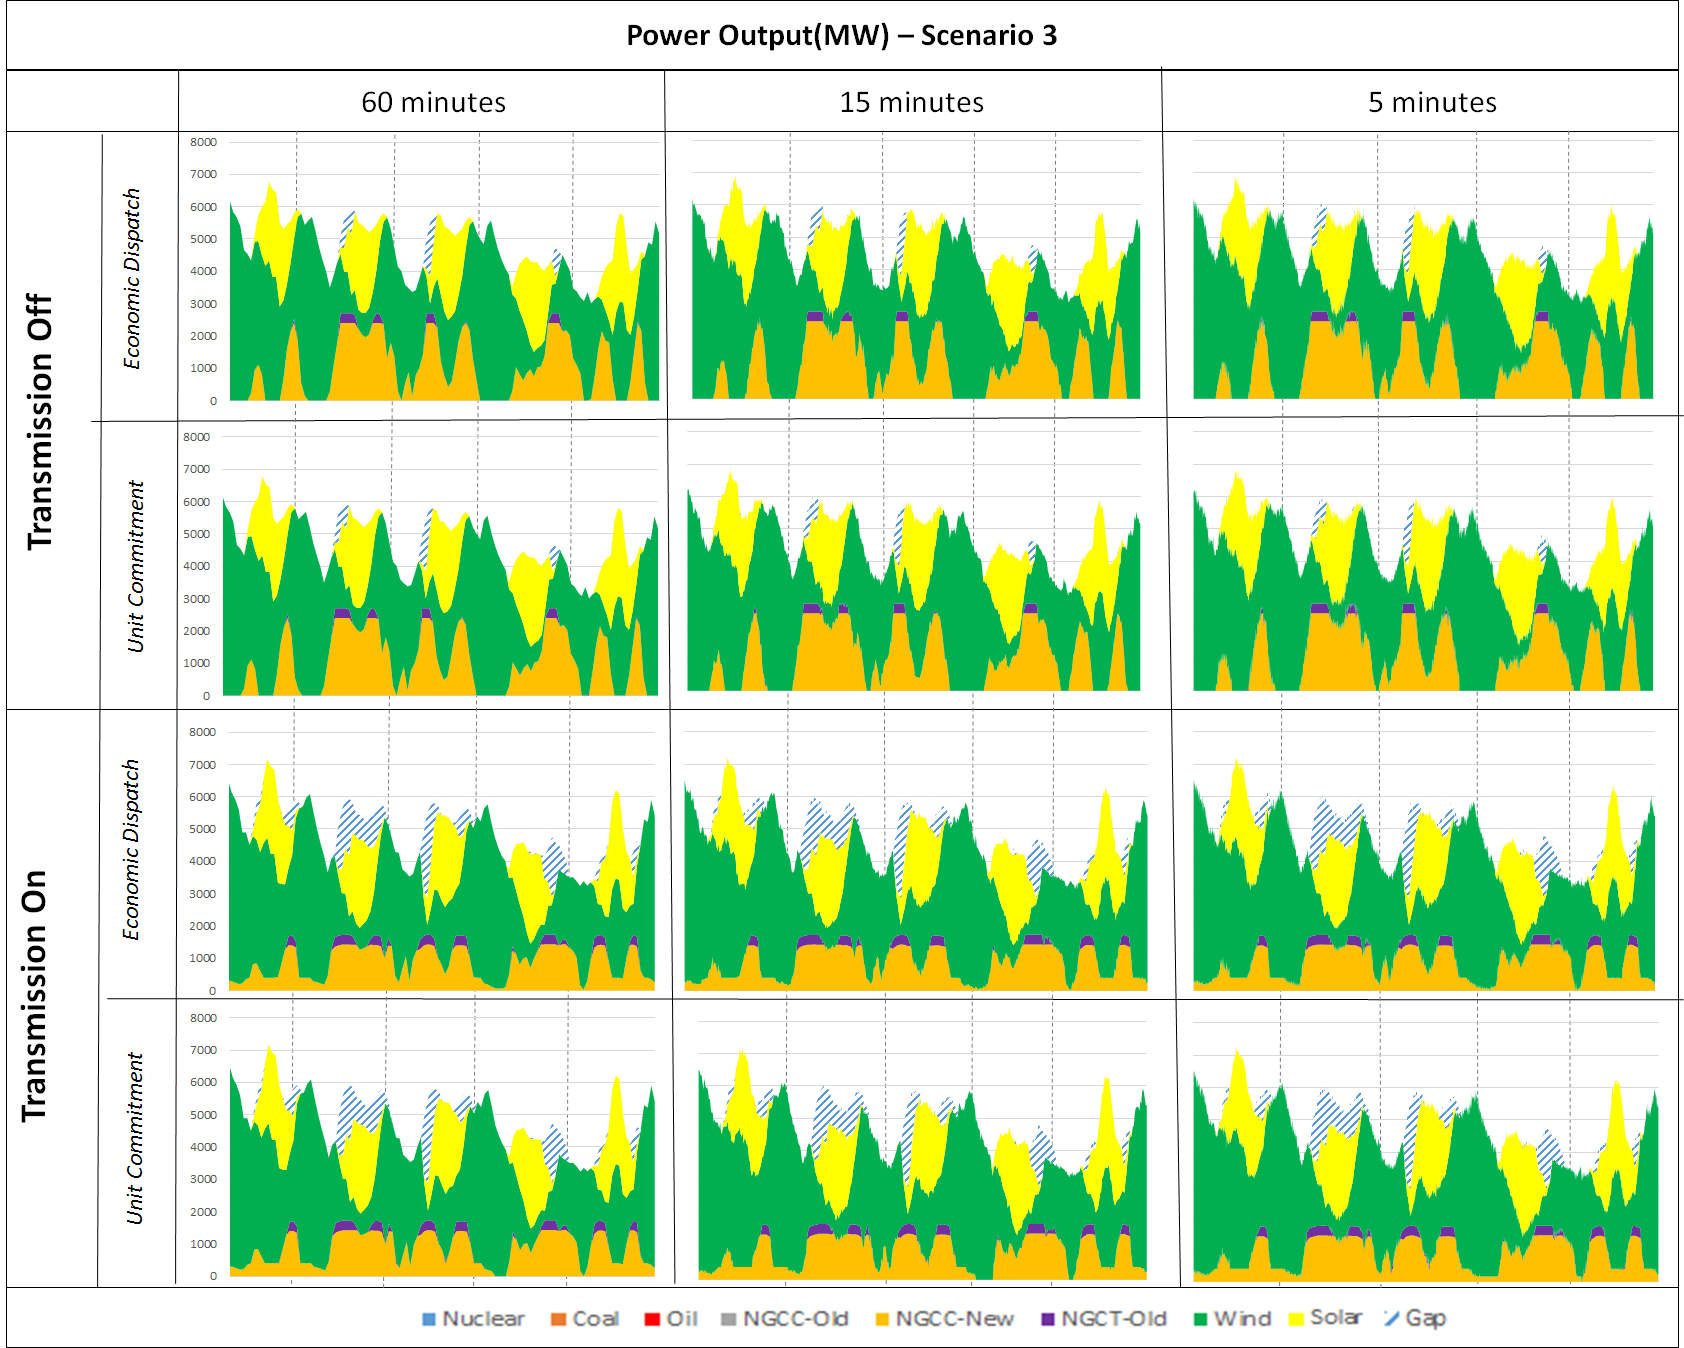
\includegraphics[width=\textwidth,height=\textheight,keepaspectratio]{PowerOutputScenario3.png}
  \caption{Power Output for Scenario 3.}
  \label{fig:powerOutputScenario3}
\end{figure}

Scenario 3 is perhaps the most challenging and uncertain set to plan, especially because of high variable resource penetration and their variability over time. In all configurations the demand was not entirely met, especially in peak hours and low wind generation. 

Also, transmission assumptions made a very important key in the power planning results: there is a considerable difference in the generation for non-renewable resources when comparing transmission on and off, for both optimization models. The transmission is a bottleneck in two cases: to fulfil the demand at peak levels and to transmit energy coming from renewable resources. 

When comparing the generation between UC and ED instances NGCC-New generators are the predominant source of NVRE, having NCTG-Old as a support to peak and low wind and solar generation moments. The UC model decided to turn on most of NGCC-Generators and keep them running at a minimal level during low demand when transmission is not consider. For the other case the generation is bounded by line transmission limits, so the solution turns on generators from other locations. Thus, although the system is able to fulfill most of the demand in Scenario 3, it is not able to transmit it.



\newpage
\subsection{Scenario 4 Storage Analysis}

\begin{figure}[H] 
	\begin{center}
		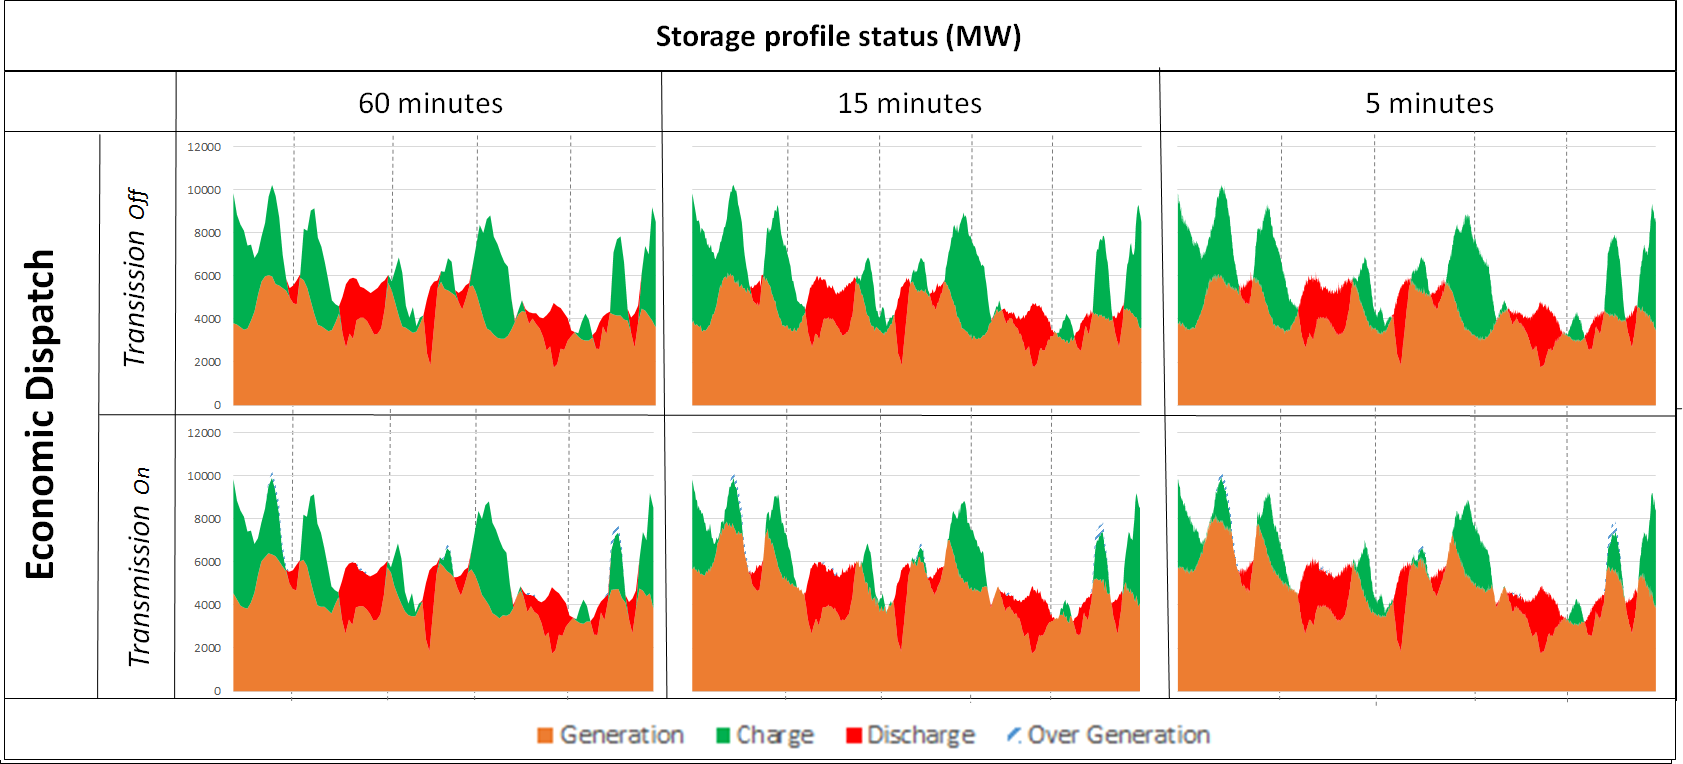
\includegraphics[width=\textwidth,keepaspectratio]{StorageProfileStatusS4.png}
	  	\caption{Storage Device Profile Status for Scenario 4.}
     	\label{fig:storageprofilestatus}
	\end{center}
\end{figure}

Scenario 4 deserves special analysis, since all the energy comes from intermittent sources and there are storage devices in the system (which was not the case in the previous scenarios). As an extreme case, for the same RTS-96 load, the objective is to use storage to avoid under-generation which can incur several penalties. One common question, which was the object of study of \citeauthor{safaei} \cite{safaei} is: how much storage is necessary in a green world to guarantee power supply? Figure \ref{fig:storageprofilestatus} displays the results of the optimization models to Economic Dispatch, segmented by 4 categories: the power generated by wind and solar, the power charged, the power discharged and the power not charged (over generation slack). Since there is no NVRE generator and it is assumed that all renewable generators are on permanently there was no reason to run this scenario under Unit Commitment instances. We observed no significant difference in between instances with or without transmission, since, in this scenario, storage devices were spread all over the network to minimize transmission limit bounds, which would be the case in ideal situations. However, it is important to mention that even with unlimited capacity there was some over generation in isolated periods, and the reason is as follows: there was an abrupt ramping in VRE generation higher than the ramping limits for the storage devices, so they were not able to store it. 

To estimate the amount of load that was satisfied by storage devices, we calculated the area of each instance described in figure \ref{fig:storageprofilestatus} of the total load (Generation + Discharge) and the Discharge curve itself, then divided both values. Figure \ref{fig:loadfilled} shows that in average nearly 47\% of the load had to be filled by storage devices, which corresponds to 4018.5 MW in a period of 7 days.

\begin{figure}[H] 
	\begin{center}
		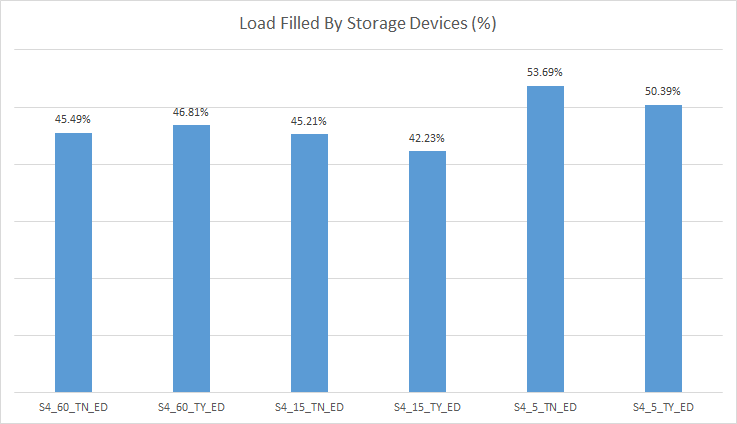
\includegraphics[width=0.6\textwidth,keepaspectratio]{loadfilledstorage.png}
	  	\caption{Percentage of Load Filled by Storage Devices per Instance.}
     	\label{fig:loadfilled}
	\end{center}
\end{figure}

\newpage
\section{Optimization Results} \label{section:optimizationresults}

Table \ref{table:modelparameters} describes the number of variables and parameters for each studied instance. 



\begin{table}[H]
\centering
\caption{Optimization Model Parameters.}
\resizebox{0.5\linewidth}{!}{%
\begin{tabular}{|l|l|l|}
\hline
Instance&Number of Variables&Number of Constraints\\
\hline
S1\_ 15\_TN\_ED&137,086&201,059\\
S1\_15\_TN\_UC&185,667 (86,580 integer)&202,382\\
S1\_15\_TY\_ED&240,982&235,691\\
S1\_15\_TY\_UC&289,563 (86,580 integer)&237,014\\
S1\_5\_TN\_ED&410,686&602,339\\
S1\_5\_TN\_UC&556,227 (259,380 integer)&606,542\\
S1\_5\_TY\_ED&721,942&706,091\\
S1\_5\_TY\_UC&867,483 (259,380 integer)&710,294\\
S1\_60\_TN\_ED&34,486&50,579\\
S1\_60\_TN\_UC&46,707 (21,780 integer)&50,822\\
S1\_60\_TY\_ED&60,622&59,291\\
S1\_60\_TY\_UC&72,843 (21,780 integer)&59,534\\
S2\_15\_TN\_ED&126,504&169,313\\
S2\_15\_TN\_UC&251,083 (135,642 integer)&260,034\\
S2\_15\_TY\_ED&230,400&203,945\\
S2\_15\_TY\_UC&354,979 (135,642 integer)&294,666\\
S2\_5\_TN\_ED&378,984&507,233\\
S2\_5\_TN\_UC&752,203 (406,362 integer)&779,394\\
S2\_5\_TY\_ED&690,240&610,985\\
S2\_5\_TY\_UC&106,3459 (406,362 integer)&883,146\\
S2\_60\_TN\_ED&31,824&42,593\\
S2\_60\_TN\_UC&63,163 (34,122 integer)&65,274\\
S2\_60\_TY\_ED&57,960&51,305\\
S2\_60\_TY\_UC&89,299 (34,122 integer)&73,986\\
S3\_15\_TN\_ED&115,441&136,124\\
S3\_15\_TN\_UC&251,083 (135,642 integer)&235,984\\
S3\_15\_TY\_ED&219,337&170,756\\
S3\_15\_TY\_UC&354,979 (135,642 integer)&270,616\\
S3\_5\_TN\_ED&345,841&407,804\\
S3\_5\_TN\_UC&752,203 (406,362 integer)&707,344\\
S3\_5\_TY\_ED&657,097&511,556\\
S3\_5\_TY\_UC&1,063,459 (406,362 integer)&811,096\\
S3\_60\_TN\_ED&29,041&34,244\\
S3\_60\_TN\_UC&63,163 (34,122 integer)&59,224\\
S3\_60\_TY\_ED&55,177&42,956\\
S3\_60\_TY\_UC&89,299 (34,122 integer)&67,936\\
S4\_15\_TN\_ED&101,973&32,184\\
S4\_15\_TY\_ED&205,869&66,816\\
S4\_5\_TN\_ED&305,493&96,504\\
S4\_5\_TY\_ED&616,749&200,256\\
S4\_60\_TN\_ED&25,653&8,064\\
S4\_60\_TY\_ED&51,789&16,776\\
\hline
\end{tabular}
}
\label{table:modelparameters}
\end{table}

Unit Commitment has many more variables than Economic Dispatch models, and reaching sub-hourly levels can lead to hundreds of thousands, even millions of variables. This affects the solution time in a non-linear way, as it can be seen in Figures \ref{fig:solutionparameterss1}, \ref{fig:solutionparameterss2} and \ref{fig:solutionparameterss3}. These graphs shows two important aspects of the optimization: the solution time and the final objective function in terms of the instance baseline for that scenario.

The UC model test was done as follows: at first, we realize it had a considerable increase in solution time when transmission constraints are active, compared to when they are not. With transmission constraints off, the solver was able to reach the integer solution with 1 \% of optimality gap (the difference between the actual solution and the linear programming relaxation) in 60-minutes, except for Scenario 1 on a 5-minute level with transmission on. In that case, even running under a 12G GB RAM memory machine, there was memory overflow. In this case the optimality MIP gap was set to 10\%. The optimal gaps for Unit Commitment instances are described better in Figure \ref{fig:mipgap}.

\begin{figure}[H] 
  \centering
	  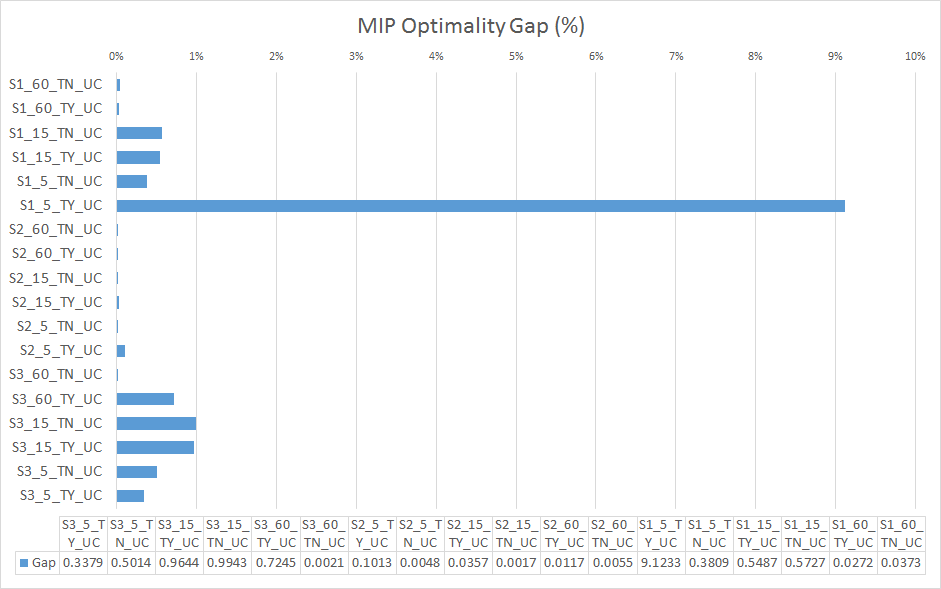
\includegraphics[width=0.7\textwidth,keepaspectratio]{mipgap.png}
  \caption{Optimality Gap for Unit Commitment Instances (\%).}
  \label{fig:mipgap}
\end{figure}


\subsubsection{Scenario 1}
In scenario 1, as expected the cheapest and fastest solution was found when no transmission is considered. It can be seen that the 15 minute level led to a better solution than ones at 60 minutes. In general, it is expected that the lower is the time granularity, the more realistic is the demand variation between the periods, making the planning more accurate. The only exception was in the instance S1\_T5\_TN\_UC, that reached a value only 0.15 \% from the baseline, but took 20 minutes to solve. 

In general the solution times for Unit Commitment are much higher than Economic Dispatch instances, due to the binary variables. However, the instance S1\_60\_TN\_UC took only 8 seconds to reach the optimal solution. The extreme case found was for the S1\_5\_TY\_UC instance, which took almost 13 hours to reach a 9\% of gap, a solution not practical either in terms of final cost and solving time.

\begin{figure}[H] 
  \centering
	  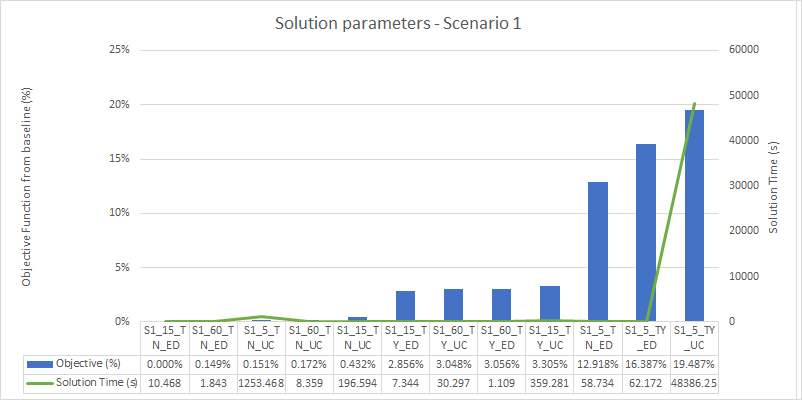
\includegraphics[width=0.8\textwidth,height=\textheight,keepaspectratio]{SolutionParametersS1.png}
  \caption{Solution Parameters - Scenario 1. Baseline: $\$658,218,352.9$.}
  \label{fig:solutionparameterss1}
\end{figure}

\subsubsection{Scenario 2}

In scenario 2 all the solutions were relatively close to each other, with the maximum solution as only 3.7 \% of the baseline. The cheapest solution was found in the instance S2\_5\_TN\_UC, indicating that, even with more demand and wind variability under sub-hourly level the solver was able to make a better plan.

It is easy to see that all the instances with transmission have a solution at least 3.5 \% of the baseline, with results similarly closer to each other. This indicates that in this case transmission limits play an important part in power planning, as was observed in figure \ref{fig:powerOutputScenario2}.

In general, Unit Commitment instances reached the optimal solutions in times closer to the ones in Scenario 1, except for the 5 minute level. The no-transmission version took 29 minutes, whereas with transmission, took almost 2 hours. So, although it seems advantageous to plan the power distribution under sub-hourly levels for this scenario, solution time can be a problem.

\begin{figure}[H] 
  \centering  
	  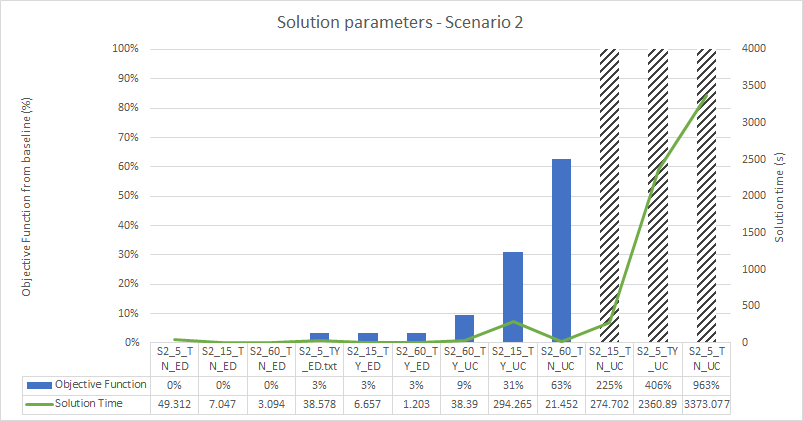
\includegraphics[width=0.8\textwidth,height=\textheight,keepaspectratio]{SolutionParametersS2.png}  
  \caption{Solution Parameters - Scenario 2. Baseline: $\$593,607,635.3$.}
  \label{fig:solutionparameterss2}
\end{figure}

\subsubsection{Scenario 3}

Scenario 3 presented different behaviour in terms of the final objective function, because of the under and over generation presented in most of instances, as observed in figure \ref{fig:powerOutputScenario3}. In terms of solution time, Scenario 3 presents better results in all instances compared to Scenarios 2 and 1. One can explain it based on the lower NVRE presence in the generation distribution, and consequently the number of decision variables. The highest solution time was set to the instance S3\_5\_TY\_UC, that took 18 minutes to solve for a weekly base. This result suggests that sub-hourly levels are more attractive to solve in this case.

\begin{figure}[H] 
  \centering
	  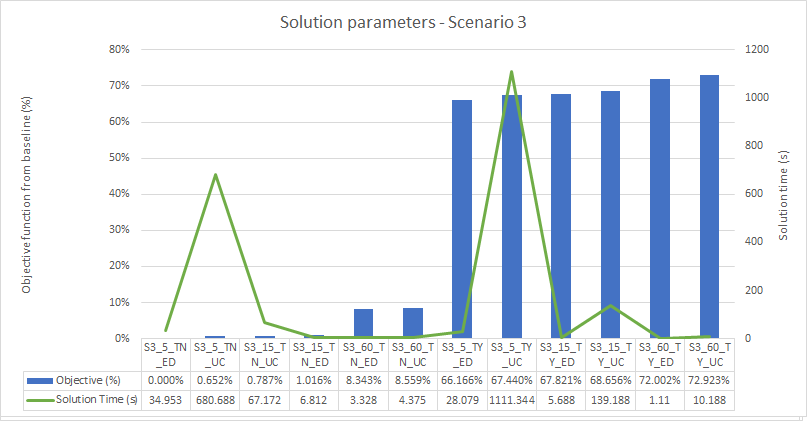
\includegraphics[width=0.8\textwidth,height=\textheight,keepaspectratio]{SolutionParametersS3.png}
  \caption{Solution Parameters - Scenario 3. Baseline: $\$264,009,305,965$.}
  \label{fig:solutionparameterss3}
\end{figure}

Recall that the penalty for the under and over generation slack variables in this case is 100,000 per MW, which explains why the baseline objective function is so large. To endorse this argument, this difference is also described by type of cost in Figure \ref{fig:genprofileS3}. It shows that gap between transmission on and off 
constraints is nearly 50 \%.

\begin{figure}[H] 
  \centering
  
	  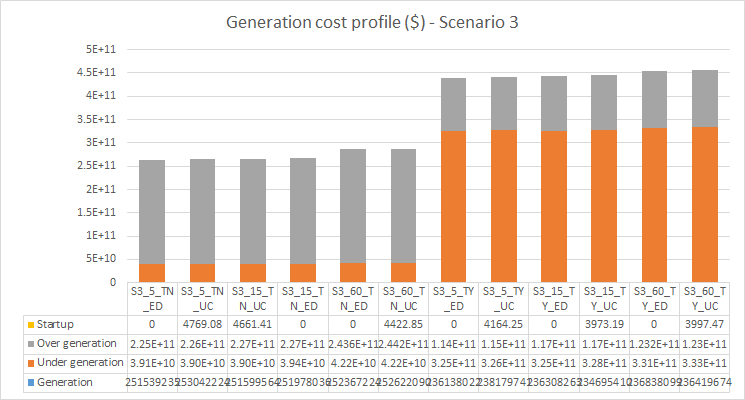
\includegraphics[width=0.8\textwidth,keepaspectratio]{genprofileS3.png}
  
  \caption{Generation Profile Cost for All Instances in Scenario 3.}
  \label{fig:genprofileS3}
\end{figure}

\newpage

\section{Transmission Results}

\begin{figure}[H] 
  \centering
  
	  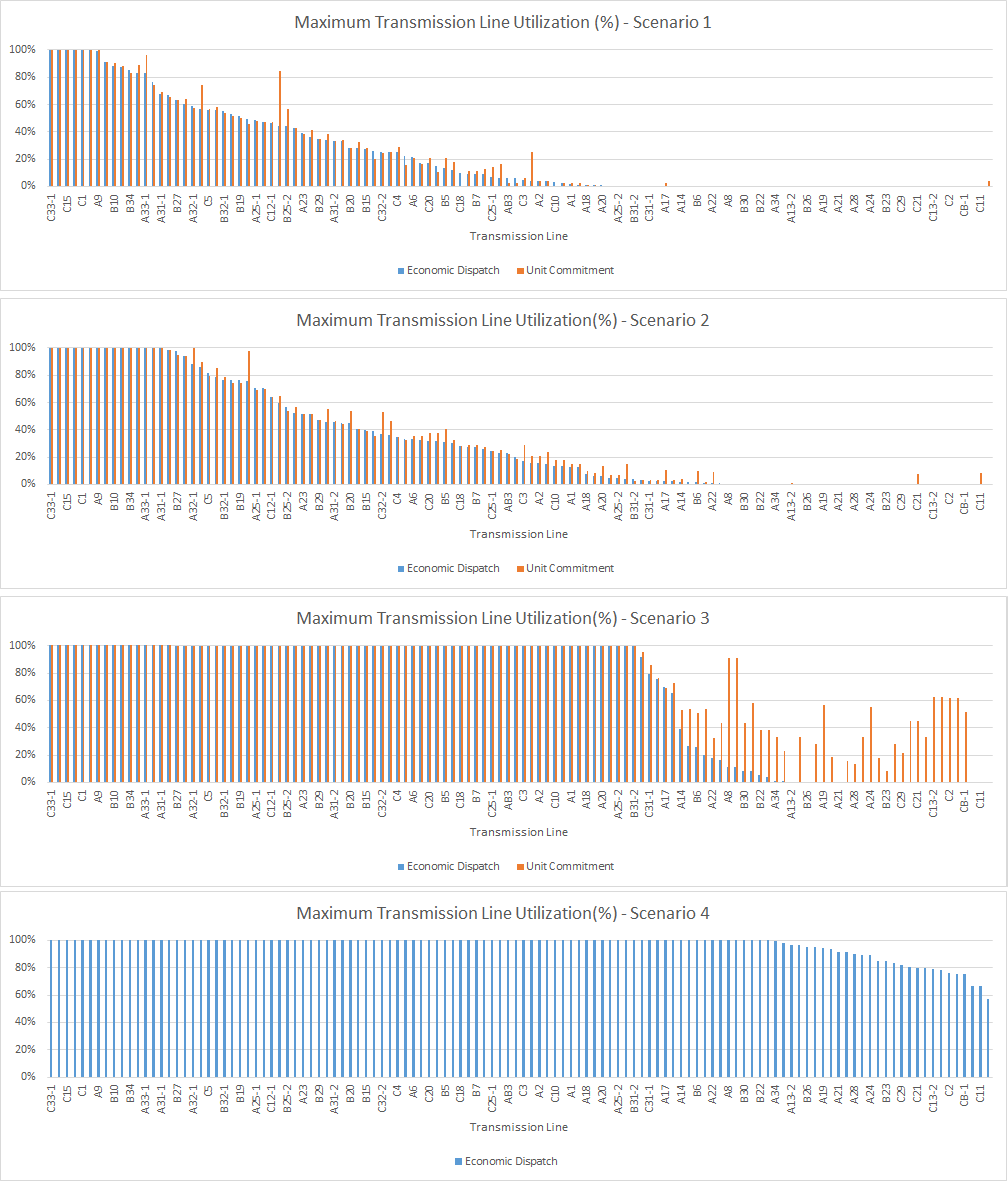
\includegraphics[width=\textwidth,height=\textheight,keepaspectratio]{MaximumTransmissionLineUtilization.png}
  
  \caption{Maximum Utilization per Transmission Line, Scenario and Model Type(\%).}
  \label{fig:maximumutilizaton}
\end{figure}

The influence of transmission constraints in the results described here depends on the distribution of generators in the field and the transmission lines physical limits. Figure \ref{fig:maximumutilizaton} shows the maximum utilization of each one of the 36 transmission lines in the field, per Unit Commitment and Economic Dispatch. 

In Scenario 1 it is clear that more than 85 \% of the transmission lines had their maximum utilization under 60\%, with 41 lines not even used for transmission.  This can be explained by the spread distribution of high capacity NVRE generators across the field, especially Oil and Coal, and the few VRE generator locations, as explained in section    \ref{section:ScenarioDesc}. It is also possible to see that Unit Commitment and Economic Dispatch instances presented nearly the same utilization behaviour, except for 7 lines. 

The same behaviour is seen in Scenario 2: low average utilization of lines and proximity between UC and ED, except for few more lines with 100\% of maximum utilization capacity. Still, this result also suggests that transmission lines are not a boundary here.

As for Scenario 3, both Unit Commitment and Economic Dispatch solutions suggests that the line is not balanced, i.e., the generators are not able to generate enough power in their locations, even though there are still lines with low or no utilization. One can state that most of the low used lines are in locations where there is no wind or solar located. Therefore, for generation capacity expansion planning, this area can be very attractive. Another aspect regarding this metric is the difference in terms of utilization between UC and ED: the line utilization for UC is 13 \% more than the ED instances. This can suggest that Unit Commitment decided to turn on and use different generations in its power planning compared to EC, and transmission limits might be a reason for that.

\section{Ramping Results} \label{section:ramping}

Another goal of this project is to evaluate the impact on non-renewable generators ramping when the power planning done at different granularities for different scenarios. The average ramping is normalized by the generator type maximum capacity. The normalization was necessary to avoid the idea of low-capacity generators ramping less than high-capacity ones. The results are displayed in figure  \ref{fig:averageramping}.

\begin{figure}[H] 
  \centering
  
	  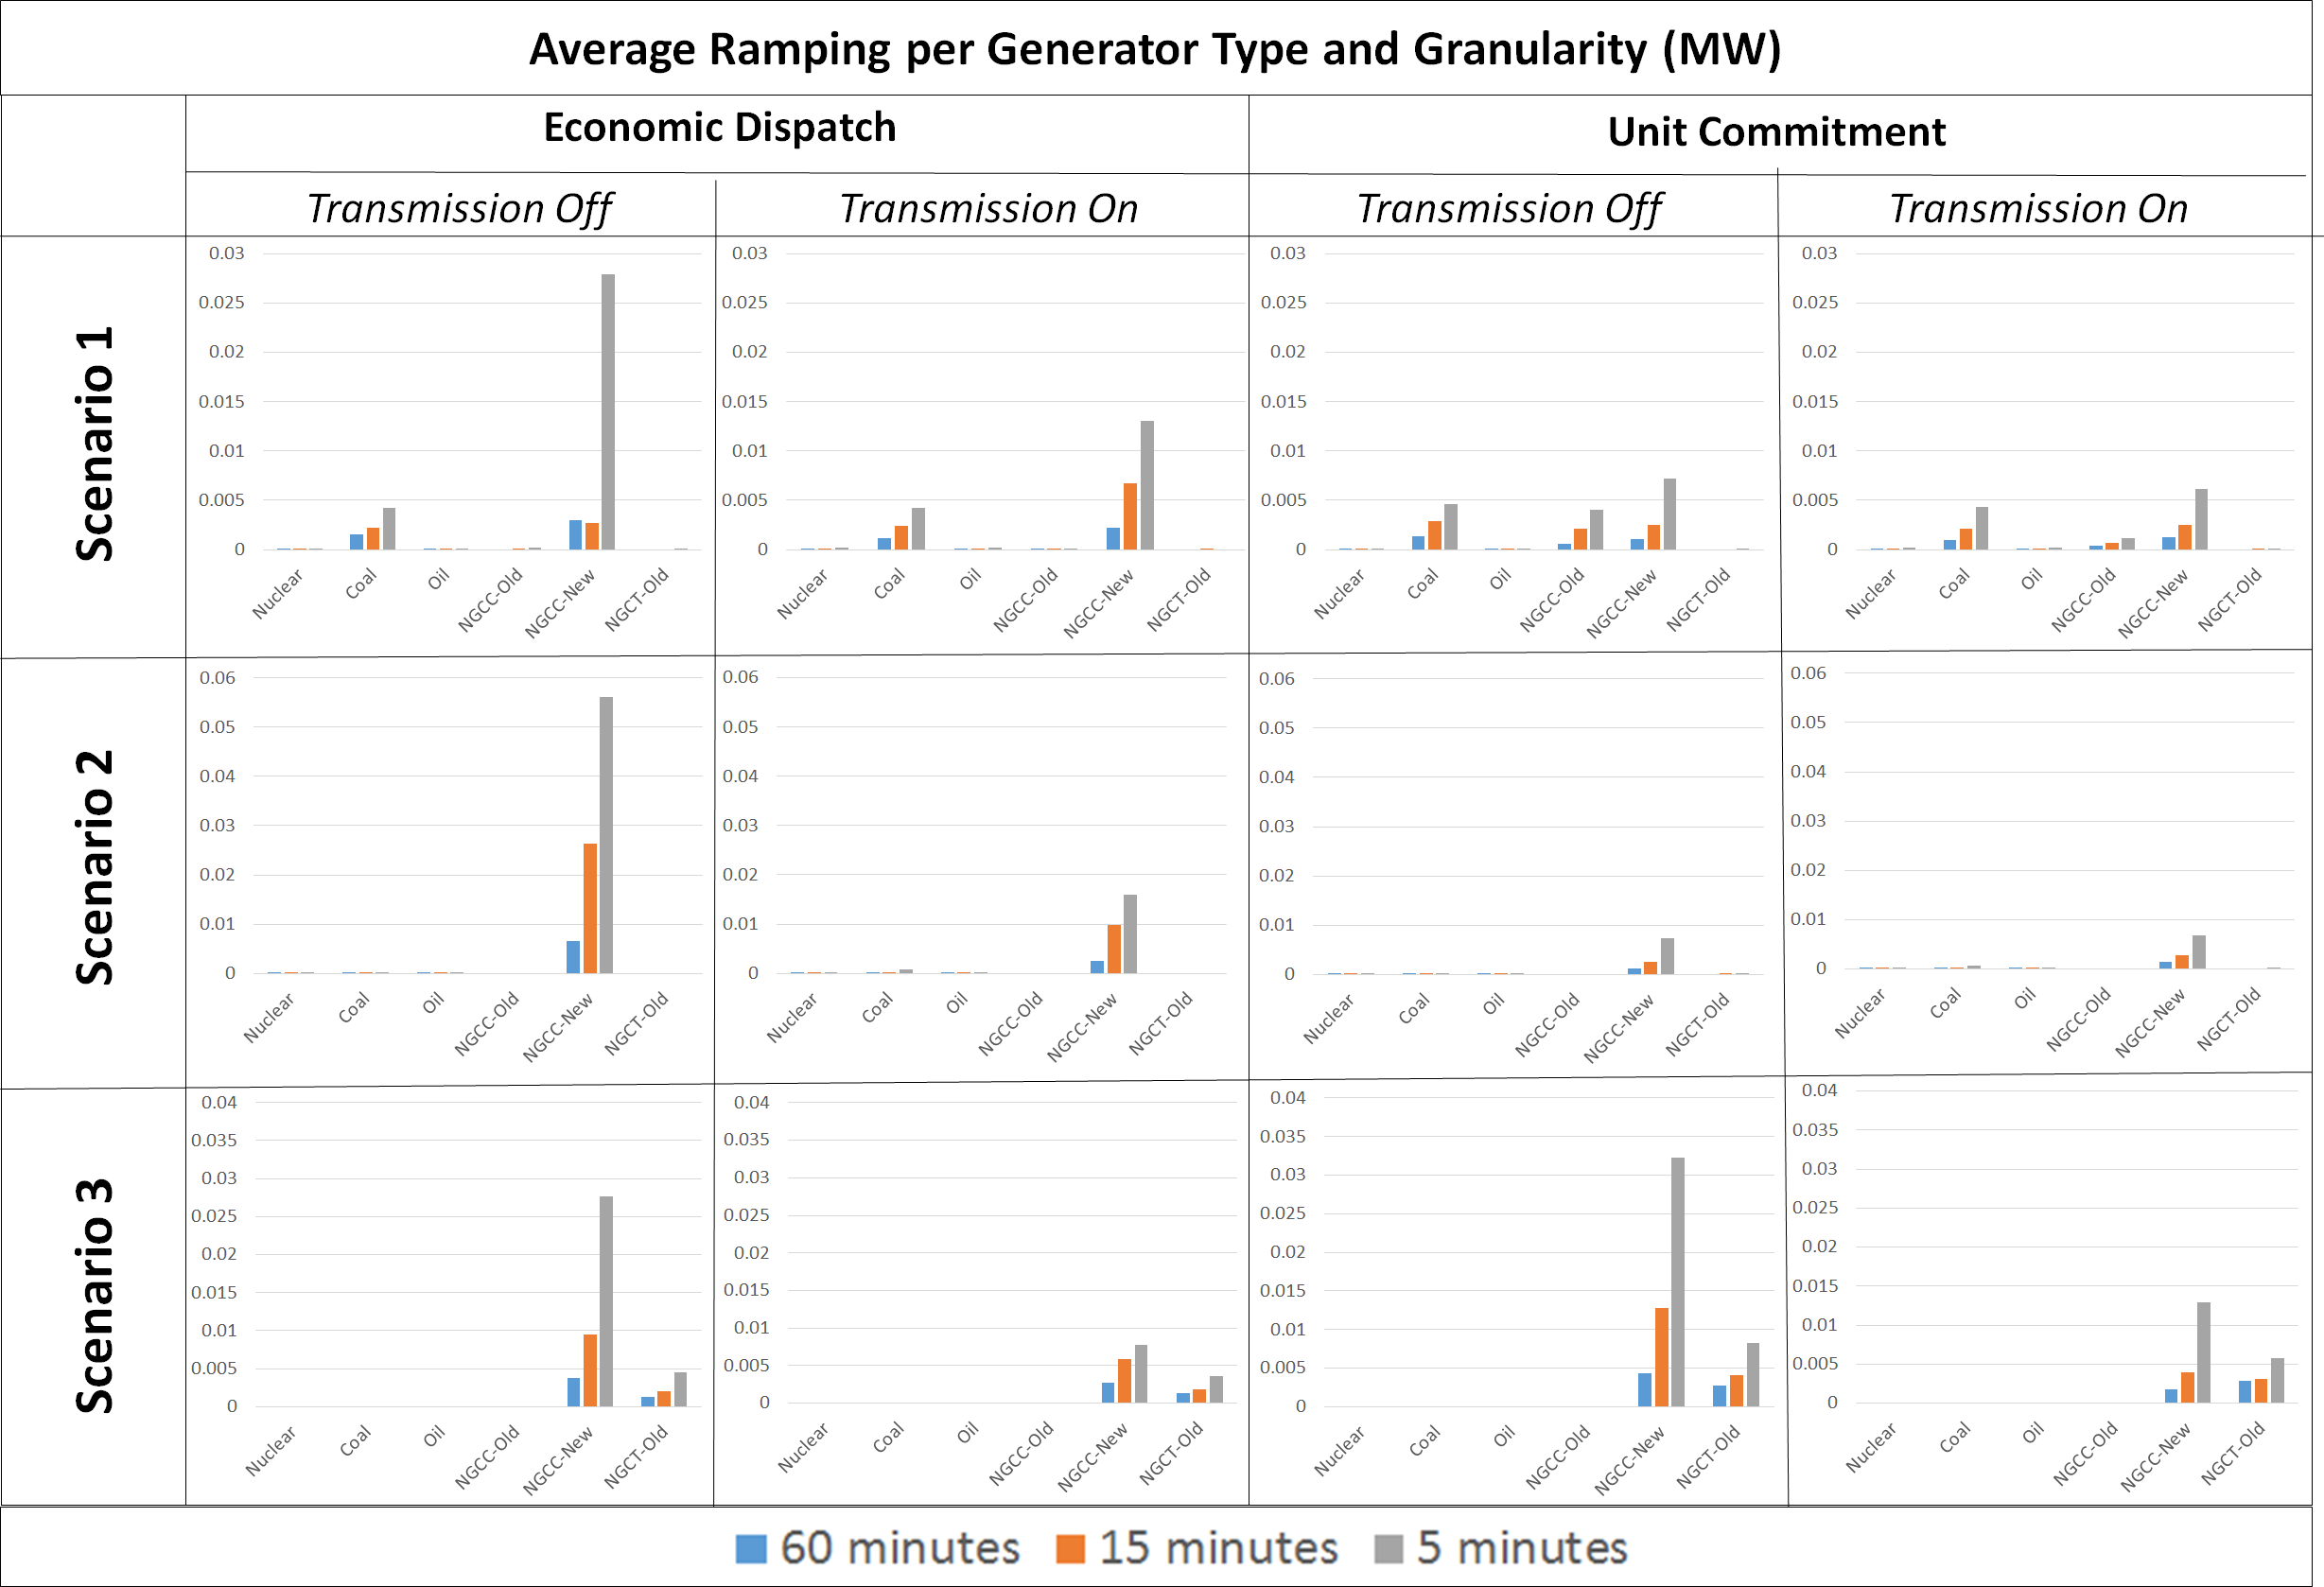
\includegraphics[width=\textwidth,height=\textheight,keepaspectratio]{averageRamping.png}
  
  \caption{Average Ramping of Non-renewable Generators, Normalized by Maximum Capacity.}
  \label{fig:averageramping}
    
\end{figure}

The ramping results for the Economic Dispatch model seem to follow a pattern: the closer is the time scale, higher is the average ramping. They also suggest that the more VREs are in the system, the more is the difference between time granularities. This result make sense; sub-hourly levels can capture the small variances in loads and the intermittence of energy sources more accurately. 

In Scenario 1 there is no significant difference between Unit Commitment and Economic Dispatch instances in terms or ramping, except in the case of NGCC-New generators. The reason for this is the absence of minimum generation in ED models and the use of this type of generator only during peak levels. The instance S1\_5\_TN\_ED generated a bigger average ramping result for NGCC-New generators. The optimal solution decided to not ramp the base generators during peak levels and let the NGCC-handle all the variabilites. Also, the fact that it is used only during peak and then it is shutdown might be another reason.
%Complete and try to explain why

In Scenario 2, although transmission is not a bottleneck in the sense that it provides generation gaps, it definitely changed the generation profile of each individual NGCC-New generator. When transmission constraints are enabled, the solution provides less intermittent generation than when it is not. This was also observed in Unit Commitment instances, as observed in figure    \ref{fig:generationProfileNGCC}. The same applies for sub-hourly planning levels. A generation profile as seen in S2\_60\_TN\_ED definitely can increase the maintenance costs, due to this constant ramps.

\begin{figure}[H] 
  \centering
  
	  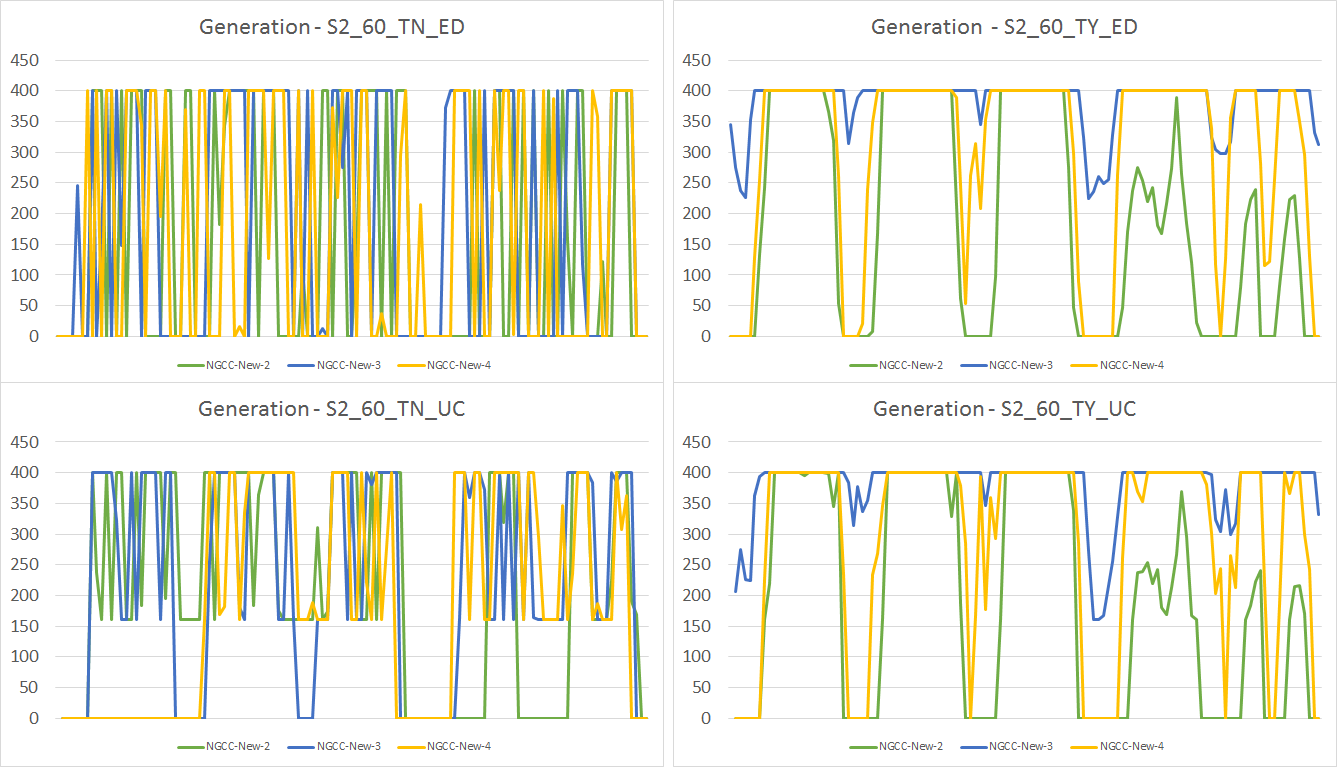
\includegraphics[width=\textwidth,keepaspectratio]{generationProfileNGCC.png}
  
  \caption{Generation Profile for 3 Individual NGCC-New Generators for a 60-minute Level.}
  \label{fig:generationProfileNGCC}
  
\end{figure}


In Scenario 3, again, the transmission bottleneck also affects the ramping capability of generators in the sense that it limits NGCC-New generators from responding to quick load and VREs variations. It is observed that the ramping profile is very similar between ED and UC instances when transmission is off. When it is on, NGCT-Old has a slight increase in its ramping, and the same is true for 5-minute level for NGCC-New generators. 

\section{Unit Commitment start-up / shutdown levels} \label{section:uconoffstatus}

The last analysis of this report discusses the start up/shutdown behavior of NVRE types provided by Unit Commitment results. Figures \ref{fig:activeGeneratorsS1}, \ref{fig:activeGeneratorsS2} and \ref{fig:activeGeneratorsS3} demonstrate the number of active generators over time.

Scenario 1 is the one that has the most different startup profile between the 6 instances. In General, the number of Oil and Nuclear active generators are set, although some minor changes were observed in peak hours for Oil. Some Coal and NGCC-New generators are shutdown in low demand times. When transmission is off, 5 NGCC-New generators were turned on during peak hours, whereas when transmission is on,, only 4. To fill this gap, in average 2 NGCC-Old generators are turned on, while NGCT-Old are used only to respond to quick unexpected ramping events.

\begin{figure}[H] 
  \centering
  
	  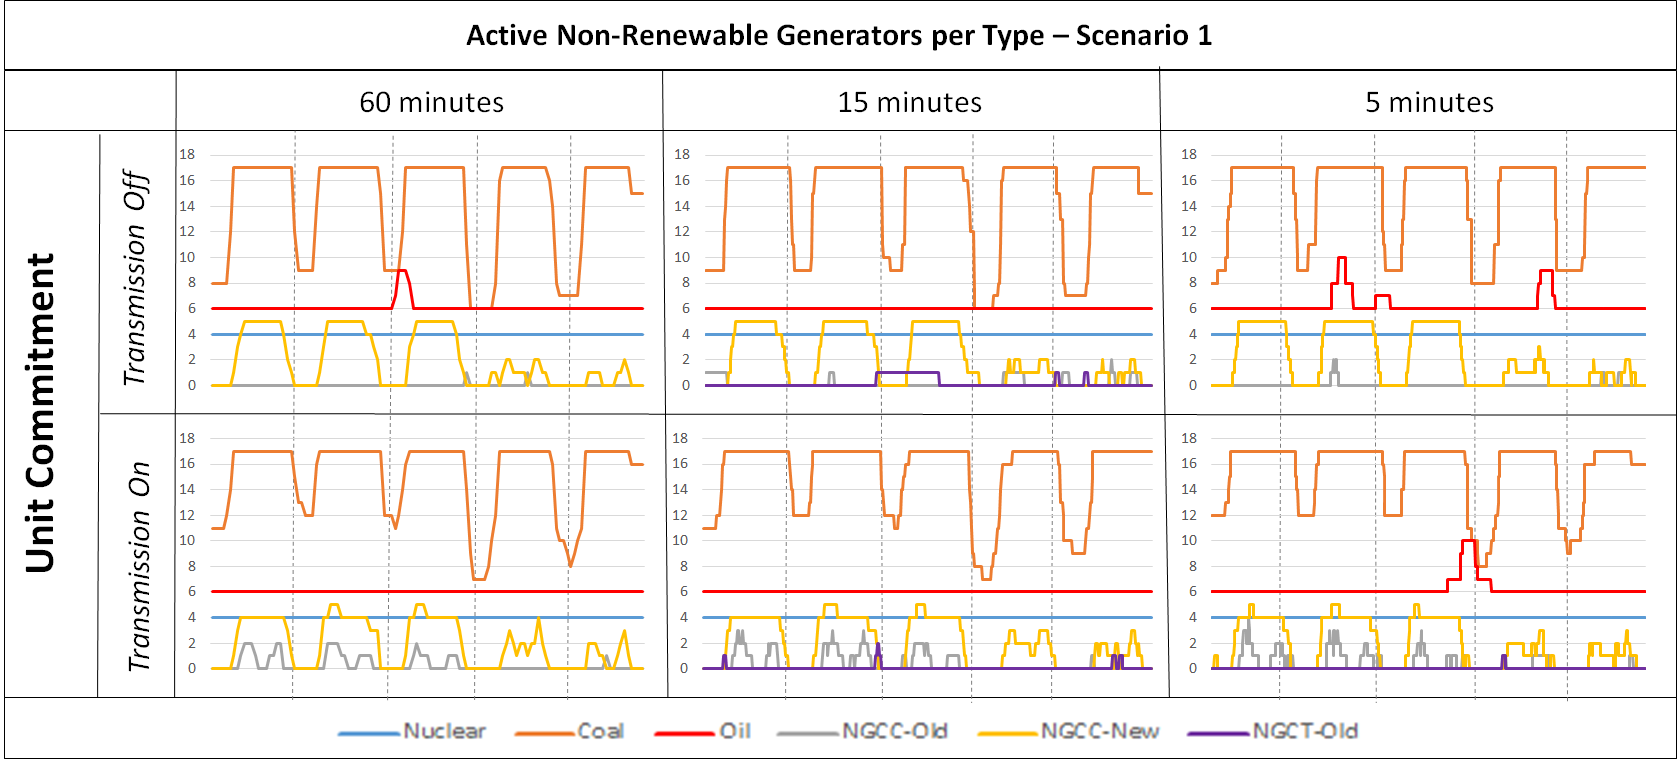
\includegraphics[width=0.8\textwidth,keepaspectratio]{activeGeneratorsS1.png}
  
  \caption{Number of Active Generators by Type over Time for Scenario 1.}
  \label{fig:activeGeneratorsS1}
  \end{figure}
  
  \begin{figure}[H] 
  \centering
  
	  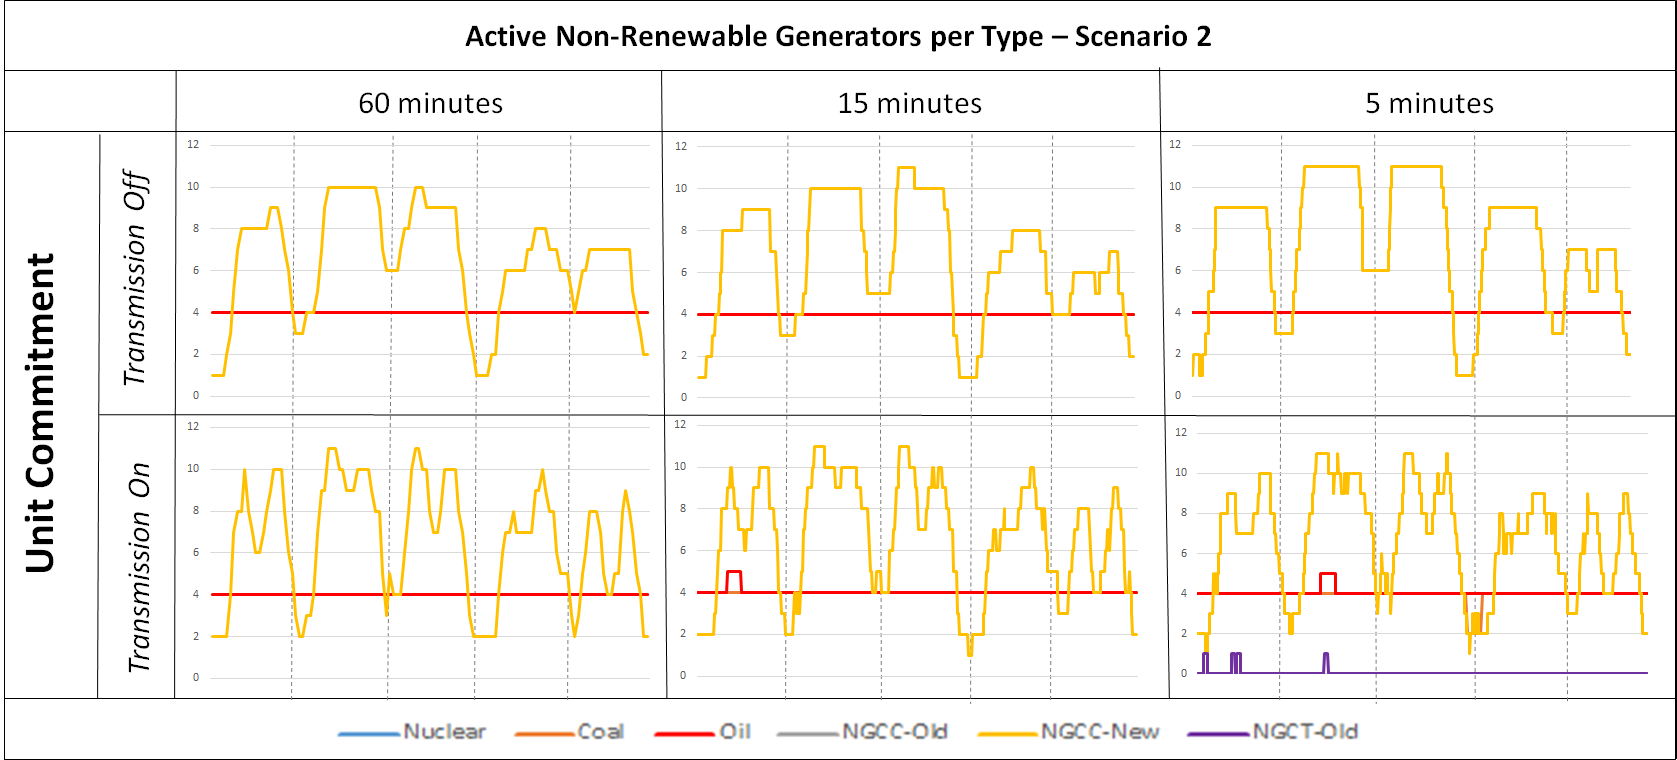
\includegraphics[width=0.8\textwidth,keepaspectratio]{activeGeneratorsS2.png}
  
  \caption{Number of Active Generators by Type over Time for Scenario 2.}
  \label{fig:activeGeneratorsS2}
  
\end{figure}


\begin{figure}[H] 
  \centering
  
	  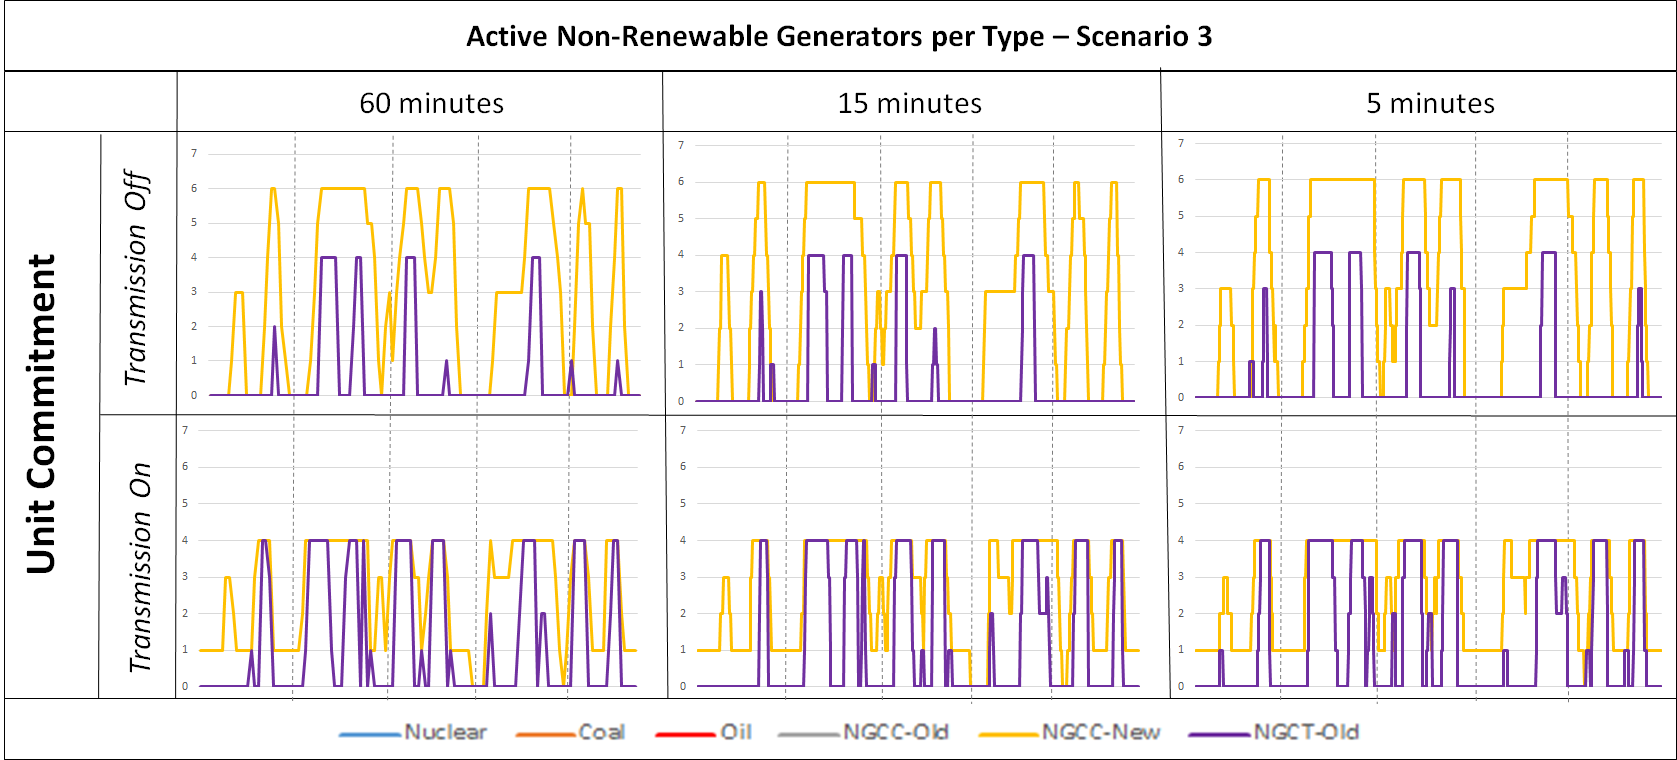
\includegraphics[width=0.8\textwidth,keepaspectratio]{activeGeneratorsS3.png}
  
  \caption{Number of Active Generators by Type over Time for Scenario 3.}
  \label{fig:activeGeneratorsS3}
  
\end{figure}

An essential difference in Scenario 2 is between time granularities, especially when transmission constraints are active. Under 15 and 5 minute levels the solution with transmission turned on and off more NGCC-New generators, respecting their minimum up and downtime, in order to fulfill sub-hourly load variability while generating at minimal cost. This incurs more start-up and shutdown costs, as well as maintenance costs. Also, we observed a minor use of NGCT-Old generators, for the same reason as Scenario 1.

In Scenario 3, the quick up and downtime requirements for gas generators allows solutions to quickly start-up and shut-down when it is convenient. It is noticed that NGCT-Old generators are activated only during peak demand, and deactivated afterwards, whereas NGCC-New are activated also in low wind and solar variability. As previously discussed, the transmission limits in this scenario limits the number of 4 NGCC-New generators running at the same time, compared to 6 when transmission is not considered.

\chapter{Conclusions}

\section{Discussions}

As discussed in the introduction, this thesis had the main objective to evaluate the impact on Unit Commitment and Economic Dispatch classic views under different configurations. The rise and necessity of the world to use more green energy rather than traditional sources could bring several challenges in terms or power planning, under different aspects, as can be observed in the Analysis section. 

In the power systems planning field, it is common to use default test cases from IEEE to test different methodologies, like power flow techniques, reliability tests and so on. However,the RTS-96 was developed 20 years ago, a time that renewable energy was just starting to emerge and be studied. That is why we decided to update the generation profile, adding more green sources not present originally in the model, like natural gas, wind and solar. All the new parameters, costs, modelling and technical details were extracted and analysed from real data and academically trusted sources. Therefore, one could argue that all the results discussed in the analysis section are valid and represent real-world power systems, on a smaller scale.

The results presented in the Analysis section could lead to the following questions:

\begin{itemize}
\item Which model should I use ?
\item What is the ideal time level ? Hourly or sub-hourly levels ?
\item What should be my planning horizon ?
\item Should I have storage or not ?
\end{itemize}

There are no easy answers for these questions. Even two simple and well-know models, are Economic Dispatch to and Unit Commitment, can lead to different results under different configurations, scenarios and perspectives, as we can see in the Analysis section. This chapter highlights some findings that might help in answering that questions.

%Economic Dispatch models in general are easier and faster to solve, but in some cases that might not apply.
The first discussion is the difference between the use of Economic Dispatch and Unit Commitment models in different VRE levels. First, sub-hourly levels instances of Economic Dispatch were able to capture with more precision the fluctuations of load demand, allowing the planner to be more specific. Also, as we were able to see in the Scenario 3, the more is the penetration of intermittent power sources, the more different is the power behaviour of non-renewable sources between different time scales. As discussed in section \ref{section:ramping}, differences in average ramping in Scenario 3 for different instances of ED suggests that hourly planning could lead to an underestimation of the ramping behaviour for NRVEs in the system. Therefore the first important conclusion is: the more VRE's in the system, more necessary is the need forpower planning at sub-hourly levels.

%Under sub-hourly levels, Unit Commitment is not efficient and, therefore, it must be used wisely.
Economic Dispatch is a model that is easy to solve since it is a LP and there is not too much complexity increase when solved under sub-hourly levels. Nevertheless the same is not true for Unit Commitment. As shown in section \ref{section:optimizationresults}, at a 5-minute level the solver took minutes, sometimes even hours to reach an acceptable gap, with a power profile generation slightly close to the hourly levels. Of course this thesis solved this problem over one week, using the traditional modelling. In a scenario of high VRE penetration, it is necessary to use smarter techniques of commiting generators rather than just solving the MIP. One of these is the rolling horizon algorithm, described by \citeauthor{tuohy} \cite{tuohy}, which divides the problem into small MIP problems, solves them in a period and uses the result as an input to solve the next one. Unit Commitment levels does not lead itself to solving under sub-hourly levels, due to the computational burden. 

There are two additional aspects regarding Unit Commitment that are important to mention. First, more generator start-ups and shut-downs were observed in Scenario 2. This incurs more maintenance and repair costs. To mitigate this, one can limit the number of start-ups and shut-downs for the study as constraints, although it would add more complexity to the model. Second, as discussed in section \ref{section:ramping}, sometimes it is necessary to understand the generation profile for each individual generator.

The proximity of solution quality between models at different time granularity indicates that it might not be a vantage to run them under a different time level on a long planning horizon. So, either runs it on a 60-minute level, or reduce the planning horizon. Under high penetration levels, the 5 minute level seems to be more reasonable to solve, and has to be considered carefully. Of course this project assumed that the wind and solar availability are deterministic parameters of the model. This can change when these variables are stochastic, or when the start-up / shut-down decisions also apply to green generators.

%\item Under-generation slack variables with a high penalty can lead to numerical instabilities and non-feasible solution times.
Another important aspect is how do deal with slack variables in the system. Although they are important to always reach a feasible solution in the planning, during our numerical runs of all the instances we faced some numerical issues with them, specially in Scenario 3. A lower penalty led the solver to choose to pay the penalty instead of turning on a generator, ramp and generate power during peak levels. On the other hand, when we set these penalties to a big value, e.g. \$ 100,000,000.00 per MW, it impacted the solver negatively in terms of solution time, specially in Unit Commitment levels. Therefore, it is necessary to estimate wisely what would be the penalty to not generate or curtail power, issues that are important under a high penetration of VREs.

%\item Transmission parameters plays an important rule in both solution times and quality, specially under high VRE levels.
From scenarios 2 and 3 and 4 , the transmission system is an important parameter that can not be neglected in the dispatch decisions, specially for quick ramp events. We noticed that, in some moments when there was an abrupt variation of wind and solar supply, although there were available generators to respond to it, their generation was bounded by transmission line limits. Therefore, in the real world transmission adds complexity to the optimization model, but overlooking it can lead to wrong planning decisions. Also, that applies to other non-linear parameters not considered in this thesis, such as reactive power, voltage angle, heat and other transmission properties. The results suggests that, in a position where solving time and computational resources are restricted, it is better to solve the model on an hourly level with transmission constraints than solving on a sub-hourly without them.

Storage devices are an important key to allow more green world penetration, either to store all the remaining generation or supply at peak time and low wind and solar demand. In the studied scenario, almost 50\% of the load was supplied from storage devices, under distributed unlimited storage capacity with a nameplate generation capacity at double the peak load. In a major scale as a real-world situation, this might not be economically feasible, due to implementation, maintenance and deployment costs of storage devices. Still, they should be definitely a feature to consider in capacity expansion planning studies. Without them it is impossible to guarantee power supply in a green world, no matter how much is the installed capacity of solar and wind resources.

\section{Future Improvements}

This project had the achievement of building a full test scenario that represents a real power planning system, with capability to explore and analyse the data intuitively under a powerful mathematical modelling tool. To make this work even more rich, the following future improvements are suggested:

\begin{itemize}
\item Implement additional power planning techniques , and evaluate them under different time planning levels. There are a lot of different advanced techniques that have proven to be useful, as discussed in the Literature Review section. One technique suggested to implement is the rolling horizon for Unit Commitment decisions.
\item Explore more the storage device scenario, and use them with expansion planning models to evaluate the impact of building them instead of generators. Also, add more constraints, such as capacity, ramping, start-up and shut-down levels, etc.
\item Explore more the transmission limits, adding more physical restrictions, like voltage angle, reactive power, transmission outage rates. Also, evaluate the transmission reliability system tests, such as the N-1 reliability test.
\item This work considered all the demand and renewable energy forecasts as accurate. A suggestion is add forecast errors, and evaluate what would be the impact of them in power planning. So it is suggested to embed a simulation factor in the developed system, and evaluate the impact over different VRE levels.
\item Also, model the costs changing over time. The beauty of UC and ED is to plan the generation according to the current costs, and they can change over the time planning.
\item Add UC and ED modelling to robust and stochastic optimization, making costs, demand and generation uncertain and evaluate it in terms of performance and solution quality.

\end{itemize}


\bibliographystyle{plainnat}
\nocite{*}
\addcontentsline{toc}{chapter}{Bibliography}
\bibliography{biblio}

%\addcontentsline{toc}{chapter}{Vita}
\chapter*{Vita}
\addcontentsline{toc}{chapter}{Vita}

Daniel Xavier Wolbert was born in 7 July of 1987 in Brazil, son of Cleber Wolbert and Mirian Xavier. He attended Universidade Federal de Minas Gerais in Brazil, graduating in December of 2010 in B.S. of Control and Automation Engineering. From 2010 to 2013, he acted as business and systems consultant at Accenture. He attended Lehigh University to obtain his M.S. in Industrial and Systems Engineering in May 2016. He was awarded as the "ISE Master's Student of The Year Award" in 2016.
\end{document}

